%===============================================================================
\chapter{Algebraic Foundations of Renormalization}
\label{ch:algebra}
%===============================================================================

\marginnote{This chapter reveals the deep algebraic structure underlying renormalization, starting with its origins in the numerical analysis of ODEs before showing how the same structure appears in quantum field theory.}

The preceding chapters developed the practical machinery for perturbation theory. We saw in the Prologue how the anharmonic oscillator develops secular terms that grow unboundedly, invalidating naive perturbation theory at late times. We saw in Chapter~\ref{ch:perturbation} how quantum field theories develop UV divergences that make loop integrals formally infinite. Both problems signal the breakdown of perturbative expansions, yet both admit systematic resolutions through renormalization group methods. This chapter reveals the deeper algebraic structure that organizes these expansions and their renormalization, showing that the same mathematical framework applies to both contexts.

\begin{itemize}
\item \textbf{Section~\ref{sec:butcher}}: The Butcher group and B-series for ODEs, where rooted trees organize perturbative solutions
\item \textbf{Section~\ref{sec:hopf_algebra}}: The Hopf algebra of Feynman graphs, showing the same structure in QFT
\item \textbf{Section~\ref{sec:riemann_hilbert}}: The Riemann-Hilbert correspondence, connecting renormalization to complex analysis through the Birkhoff decomposition
\item \textbf{Section~\ref{sec:hopf_resurgence}}: Connection to resurgent structure, showing how the algebraic picture complements the analytic one
\end{itemize}

The key insight is that renormalization is not an ad hoc procedure for canceling infinities. Rather, it is a mathematically natural operation with deep algebraic structure. This structure was first discovered by Butcher (1963) in the context of numerical methods for ODEs, and was later recognized by Connes and Kreimer (1998--2000) to be the same structure governing renormalization in quantum field theory.

\marginnote{Connes and Kreimer (1999) wrote of Butcher's work on numerical integration methods as ``an impressive example that concrete problem-oriented work can lead to far-reaching conceptual results.''}

%-------------------------------------------------------------------------------
\section{The Butcher Group: Hopf Algebras from ODEs}
\label{sec:butcher}
%-------------------------------------------------------------------------------

In the Prologue, we encountered perturbative corrections to the anharmonic oscillator solution that involved increasingly complicated nested time derivatives. Each higher order in the expansion required computing derivatives of derivatives, with the nonlinear terms generating ever more intricate patterns of differentiation. The natural question arises as to how we can systematically organize these nested operations and ensure that we account for all contributions at each order. This section introduces rooted trees as the mathematical structure that provides exactly this organizational framework.

The power of this approach extends far beyond the anharmonic oscillator. The same algebraic structure appears in numerical integration methods, in the perturbative expansion of general dynamical systems, and ultimately in quantum field theory. Understanding how trees organize perturbative expansions for ordinary differential equations prepares us to recognize the identical pattern in Feynman diagram calculations. We begin with the simplest setting where this structure manifests itself naturally.

\marginnote{Rooted trees encode how nested differentiations combine when we expand solutions order by order in perturbation theory.}

\subsection{Rooted Trees and Elementary Differentials}
\label{sec:rooted_trees}

Consider the autonomous ODE
\begin{equation}
\frac{dx}{ds} = f(x), \qquad x(0) = x_0
\label{eq:autonomous_ode}
\end{equation}
where $x \in \mathbb{R}^N$ and $f \in \mathbb{R}^N \to \mathbb{R}^N$ is smooth. When we expand the solution as a Taylor series in time $s$, we need to compute successive derivatives of $x(s)$. The first derivative is simply $f(x_0)$. The second derivative requires applying the chain rule to get $(Df) \cdot f$ where $Df$ is the Jacobian matrix. The third derivative involves yet more applications of the chain rule, generating terms with both second derivatives and products of first derivatives. The combinatorial complexity grows rapidly, and keeping track of all terms becomes challenging. The key observation, dating back to Cayley in 1857, is that these higher derivatives are naturally indexed by combinatorial objects called rooted trees.

\marginnote{John C. Butcher introduced the algebraic theory of Runge-Kutta methods in 1963. The infinite-dimensional Lie group of characters was identified by Hairer and Wanner in 1974 and is now called the Butcher group.}

\begin{definition}[Rooted Tree]
A rooted tree is a connected graph with no cycles and a distinguished node called the root. The number of nodes in a tree $t$ is denoted $|t|$. We denote the single-node tree containing just a root by $\bullet$.
\end{definition}

The first few rooted trees are shown below, organized by the number of nodes they contain. At each order, the number of distinct tree structures grows rapidly according to a well-known combinatorial sequence. These trees provide a natural indexing system for the terms that appear when we expand the solution of a differential equation in a Taylor series.

\marginnote{There are 1, 1, 2, 4, 9, 20, 48, 115 rooted trees with $n = 1, 2, 3, 4, 5, 6, 7, 8$ nodes respectively. This is OEIS sequence A000081.}

\begin{center}
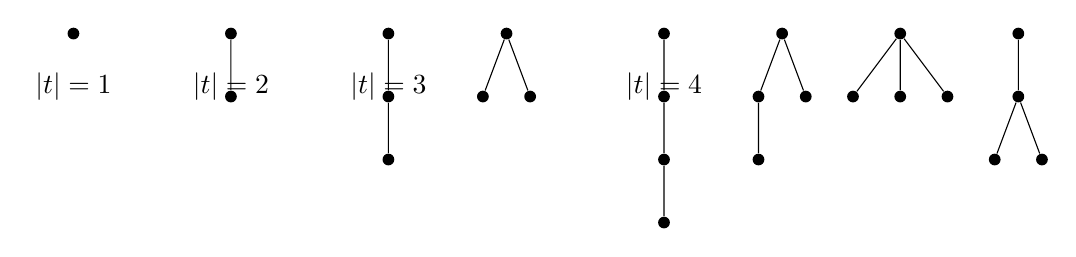
\begin{tikzpicture}[
    level distance=8mm,
    sibling distance=6mm,
    every node/.style={circle,fill,inner sep=1.5pt}
]
% n=1
\node[label=below:{$|t|=1$}] at (0,0) {};

% n=2
\node[label=below:{$|t|=2$}] at (2,0) {}
  child {node {}};

% n=3: two trees
\node[label=below:{$|t|=3$}] at (4,0) {}
  child {node {}
    child {node {}}
  };
\node at (5.5,0) {}
  child {node {}}
  child {node {}};

% n=4: four trees  
\node[label=below:{$|t|=4$}] at (7.5,0) {}
  child {node {}
    child {node {}
      child {node {}}
    }
  };
\node at (9,0) {}
  child {node {}
    child {node {}}
  }
  child {node {}};
\node at (10.5,0) {}
  child {node {}}
  child {node {}}
  child {node {}};
\node at (12,0) {}
  child {node {}
    child {node {}}
    child {node {}}
  };
\end{tikzpicture}
\end{center}

Given a tree $t = [t_1, t_2, \ldots, t_k]$ formed by attaching the roots of subtrees $t_1, \ldots, t_k$ to a new common root, we can define a corresponding differential operator. This operator, called the elementary differential, extracts exactly the coefficient of $s^{|t|}/|t|!$ in the Taylor expansion of the solution. The definition is recursive, building up complicated derivatives from simpler ones in a way that mirrors the tree structure.

\begin{definition}[Elementary Differential]
For a vector field $f \in \mathbb{R}^N \to \mathbb{R}^N$, the elementary differentials $\delta_t(x)$ are defined recursively by
\begin{align}
\delta_\bullet^i(x) &= f^i(x) \\
\delta_{[t_1, \ldots, t_k]}^i(x) &= \sum_{j_1, \ldots, j_k = 1}^N \left(\delta_{t_1}^{j_1}(x) \cdots \delta_{t_k}^{j_k}(x)\right) \frac{\partial^k f^i}{\partial x^{j_1} \cdots \partial x^{j_k}}(x)
\end{align}
\end{definition}

Each rooted tree encodes a specific pattern of nested differentiations that arise when computing time derivatives of the solution. The root corresponds to the outermost function evaluation of $f$, and each subtree corresponds to taking a derivative with respect to one argument, then substituting another instance of $f$ into that argument. This structure captures exactly how the chain rule operates when applied repeatedly. For the single-node tree, we simply evaluate $f$ at the current point. For more complicated trees, we take derivatives of $f$ and contract them with elementary differentials corresponding to the subtrees.

\begin{workedbox}[Box 7.1: Elementary Differentials for the Anharmonic Oscillator]
\textbf{Goal:} Compute elementary differentials explicitly for the damped anharmonic oscillator from the Prologue and connect them to the time derivatives that appear in perturbation theory.

\textbf{Setup:} The damped anharmonic oscillator $\ddot{x} + 2\gamma\dot{x} + \omega_0^2 x + \epsilon x^3 = 0$ can be written as a first-order system. Define the state vector $\mathbf{z} = (x, v)^T$ where $v = \dot{x}$. The vector field is then
\begin{equation}
f(\mathbf{z}) = \begin{pmatrix} v \\ -2\gamma v - \omega_0^2 x - \epsilon x^3 \end{pmatrix}
\end{equation}
At $t=0$ we take initial conditions $\mathbf{z}_0 = (A, 0)^T$, corresponding to starting at maximum displacement with zero velocity.

\textbf{The single-node tree $\bullet$:} This simply evaluates the vector field, giving the first time derivative.
\begin{equation}
\delta_\bullet(\mathbf{z}) = f(\mathbf{z}) = \begin{pmatrix} v \\ -2\gamma v - \omega_0^2 x - \epsilon x^3 \end{pmatrix}
\end{equation}
At the initial point, $\delta_\bullet(\mathbf{z}_0) = (0, -\omega_0^2 A - \epsilon A^3)^T$. The first component gives $\dot{x}(0) = 0$ and the second gives $\ddot{x}(0) = -\omega_0^2 A - \epsilon A^3$, exactly as expected from the equation of motion.

\textbf{The two-node tree $[\bullet]$:} This computes the second time derivative by applying the chain rule.
\begin{equation}
\delta_{[\bullet]}^i = \sum_j f^j \frac{\partial f^i}{\partial z^j}
\end{equation}
We need the Jacobian matrix
\begin{equation}
Df = \begin{pmatrix} \partial_x v & \partial_v v \\ \partial_x(-2\gamma v - \omega_0^2 x - \epsilon x^3) & \partial_v(-2\gamma v - \omega_0^2 x - \epsilon x^3) \end{pmatrix} = \begin{pmatrix} 0 & 1 \\ -\omega_0^2 - 3\epsilon x^2 & -2\gamma \end{pmatrix}
\end{equation}
For the $x$ component (where $i=1$), we get
\begin{equation}
\delta_{[\bullet]}^1 = v \cdot 0 + (-2\gamma v - \omega_0^2 x - \epsilon x^3) \cdot 1 = -2\gamma v - \omega_0^2 x - \epsilon x^3
\end{equation}
This is exactly $\ddot{x}$ as computed from the original equation. For the $v$ component (where $i=2$), the calculation gives $\dddot{x}$ expressed in terms of the state variables.

\textbf{The three-node fork $[\bullet, \bullet]$:} This involves second derivatives of $f$.
\begin{equation}
\delta_{[\bullet,\bullet]}^i = \sum_{j,k} f^j f^k \frac{\partial^2 f^i}{\partial z^j \partial z^k}
\end{equation}
For the $v$ component, the only nonzero second derivative is $\partial_x^2 f^2 = -6\epsilon x$. This gives
\begin{equation}
\delta_{[\bullet,\bullet]}^2 = v \cdot v \cdot (-6\epsilon x) = -6\epsilon x v^2
\end{equation}
This term represents how the cubic nonlinearity affects the third time derivative of $x$. Notice that it involves both position and velocity, reflecting the nonlinear coupling in the system.

\textbf{Key insight:} Each tree corresponds to a specific term in the perturbative expansion. The single-node tree gives the linear dynamics. Trees with more nodes incorporate the nonlinear term $\epsilon x^3$ through progressively higher derivatives. The tree structure automatically organizes how these contributions combine, ensuring we account for all terms at each order in $\epsilon$ without double counting or missing any contributions.
\end{workedbox}

\subsection{B-Series and the Taylor Expansion of Solutions}
\label{sec:bseries}

Having established that elementary differentials correspond to time derivatives at different orders, we now connect these tree-indexed quantities to the actual Taylor series solution. The remarkable fact discovered by Butcher is that the entire Taylor series can be written as a sum over rooted trees, with each tree contributing a specific term determined by its elementary differential and a combinatorial factor. This organization automatically accounts for all the complicated bookkeeping that arises from repeated application of the chain rule.

For the differential equation $\dot{x} = f(x)$ with $x(0) = x_0$, we can formally write
\begin{equation}
x(s) = x_0 + s\dot{x}(0) + \frac{s^2}{2!}\ddot{x}(0) + \frac{s^3}{3!}\dddot{x}(0) + \cdots
\end{equation}
Each time derivative can be expressed in terms of elementary differentials evaluated at $x_0$. The first derivative is simply $f(x_0) = \delta_\bullet(x_0)$. The second derivative is $(Df) \cdot f$ evaluated at $x_0$, which equals $\delta_{[\bullet]}(x_0)$. Higher derivatives involve sums of multiple tree contributions. The B-series theorem makes this structure explicit and systematic.

\begin{theorem}[B-Series Expansion]
The formal solution of $\dot{x} = f(x)$ with $x(0) = x_0$ is
\begin{equation}
x(s) = x_0 + \sum_{\text{trees } t} \frac{s^{|t|}}{\sigma(t)} \delta_t(x_0)
\label{eq:bseries}
\end{equation}
where the sum runs over all rooted trees $t$. The quantity $\sigma(t)$ is the symmetry factor of the tree, equal to the order of its automorphism group times appropriate factorial factors.
\end{theorem}

\marginnote{The symmetry factor $\sigma(t)$ accounts for equivalent ways of building the same tree, analogous to symmetry factors in Feynman diagrams.}

The symmetry factor $\sigma(t)$ prevents overcounting when multiple trees give the same contribution. For example, the fork tree $[\bullet, \bullet]$ has two identical subtrees, so permuting them does not create a distinct tree. The factor $\sigma([\bullet,\bullet]) = 2$ accounts for this redundancy. More generally, $\sigma(t)$ equals the product of factorials of the multiplicities of identical subtrees, times $|t|!$ divided by appropriate combinatorial factors. This ensures that when we sum over all trees, each distinct differential operator contribution appears with the correct coefficient.

The B-series provides a universal framework that encompasses several important applications in numerical analysis and dynamical systems. For exact solutions, it expands the exponential map from the Lie algebra to the Lie group. For Runge-Kutta methods, different choices of coefficients correspond to different approximations where only certain trees are included. For composition of flows, the B-series structure reveals how solutions at different times are related. The algebraic properties we develop next make all these connections systematic and computable.

\textbf{Connection to the Prologue:} The perturbative solution of the damped anharmonic oscillator from the Prologue can be written as a B-series. Each tree corresponds to a specific pattern of interactions between the linear part $f_0$ and the nonlinear part $\epsilon f_1$ of the vector field. To see which trees contribute at order $\epsilon^n$, we count how many times the nonlinear part appears as a vertex in the tree. Trees with no $f_1$ vertices give the linear solution. Trees with one $f_1$ vertex give order $\epsilon$ corrections. Trees with two $f_1$ vertices give order $\epsilon^2$ corrections, and so on.

Secular terms arise when certain tree contributions grow unboundedly in time rather than remaining bounded. For the anharmonic oscillator, these problematic trees have a specific structure involving resonant interactions between $f_0$ and $f_1$. When the linear frequency $\omega_0$ appears in denominators from $f_0$ vertices, and the nonlinear term produces forcing at the same frequency, the elementary differential develops factors of $t$ that grow without bound. The tree structure makes it possible to identify these secular trees systematically and organize their removal through renormalization.

\subsection{The Hopf Algebra of Rooted Trees}
\label{sec:hopf_trees}

The B-series expansion organizes individual solutions, but dynamical systems require us to compose operations in systematic ways. Consider evolving a system from initial time $t_0$ to final time $t_2$ along two possible routes. We could integrate directly from $t_0$ to $t_2$ in one step. Alternatively, we could integrate from $t_0$ to an intermediate time $t_1$, then from $t_1$ to $t_2$. These two procedures must give the same answer because the differential equation has a unique solution. This consistency requirement imposes strong constraints on how tree contributions combine and decompose.

The mathematical structure that encodes these composition rules is called a Hopf algebra. Rather than introducing this as abstract algebra, we can derive it by asking how B-series coefficients must behave under composition. When we compose two flows, trees from the first evolution combine with trees from the second evolution to produce the net result. The coproduct operation makes this decomposition explicit. When we need to invert a flow or undo a transformation, we need an inverse operation. The antipode provides this inverse. Together, these structures ensure consistency of the perturbative expansion under all the operations we might perform on solutions.

\marginnote{A Hopf algebra combines multiplication (for forming forests) with comultiplication (for decomposing trees) in a compatible way, plus an inverse operation (the antipode).}

The formal definition packages these physical requirements into algebraic language. Every physical operation translates to an algebraic operation, and the Hopf algebra axioms guarantee that everything works consistently. We now state the definition precisely, then explain each piece in physical terms.

\begin{definition}[Hopf Algebra $\mathcal{H}_R$ of Rooted Trees]
Let $\mathcal{H}_R$ be the polynomial algebra over $\mathbb{C}$ generated by rooted trees, equipped with the following structures.

\textbf{Product:} The product is the disjoint union of trees (forming a forest).
\begin{equation}
t_1 \cdot t_2 = t_1 \sqcup t_2
\end{equation}
The unit is the empty forest $\mathbf{1}$.

\textbf{Coproduct:} The coproduct $\Delta$ encodes how trees can be cut into pieces.
\begin{equation}
\Delta(t) = t \otimes \mathbf{1} + \mathbf{1} \otimes t + \sum_{\text{admissible cuts } c} P^c(t) \otimes R^c(t)
\label{eq:tree_coproduct}
\end{equation}
Here $P^c(t)$ is the pruned part (subtrees removed by the cut) and $R^c(t)$ is the remainder (what stays attached to the root).

\textbf{Counit:} The counit satisfies $\varepsilon(t) = 0$ for any non-empty tree and $\varepsilon(\mathbf{1}) = 1$.

\textbf{Antipode:} Defined recursively by
\begin{equation}
S(t) = -t - \sum_{\text{cuts } c} S(P^c(t)) \cdot R^c(t)
\label{eq:tree_antipode}
\end{equation}
\end{definition}

The product operation represents having multiple independent subsystems evolving simultaneously. When we form $t_1 \cdot t_2$, we are considering both tree contributions present but not interacting. This gives a forest rather than a single tree. The unit element represents doing nothing, the identity transformation that leaves the system unchanged.

The coproduct encodes how a composite operation can be factored into simpler pieces. When we cut a tree $t$ into pruned part $P^c(t)$ and remainder $R^c(t)$, we are asking which elementary differentials from an intermediate point combine to produce the final result. The term $t \otimes \mathbf{1}$ says we could do the entire operation at once. The term $\mathbf{1} \otimes t$ says the operation happens entirely in the second step with no preparation. The sum over cuts represents all the ways to split the work between two consecutive steps. This structure ensures that composing flows is consistent with the B-series expansion.

The antipode generates the inverse operation. Given a transformation encoded by tree $t$, the antipode $S(t)$ gives the transformation that undoes it. The recursive formula shows that to invert a complicated operation, we must first invert all its sub-operations, then combine these inversions appropriately with the remainder. This is exactly the structure needed for systematic removal of unwanted terms in perturbation theory. When secular terms appear with certain tree structures, the antipode tells us exactly what counterterm to subtract.

\begin{workedbox}[Box 7.2: The Coproduct for Small Trees]
\textbf{Goal:} Compute the coproduct explicitly for trees with 1, 2, and 3 nodes and interpret each term physically as a way of factoring the time evolution.

\textbf{Single node $\bullet$:} No non-trivial cuts are possible because there are no edges to cut.
\begin{equation}
\Delta(\bullet) = \bullet \otimes \mathbf{1} + \mathbf{1} \otimes \bullet
\end{equation}
This tree is called primitive because it cannot be decomposed into smaller pieces. Physically, this means the elementary differential $\delta_\bullet = f$ represents an atomic operation that cannot be split. The first term $\bullet \otimes \mathbf{1}$ says we could apply $f$ entirely in the first step with nothing left for the second step. The second term $\mathbf{1} \otimes \bullet$ says we do nothing in the first step and apply $f$ entirely in the second step. There is no way to genuinely split this single operation between two time intervals.

\textbf{Two nodes $[\bullet]$:} One cut is possible, separating the root from its single child.
\begin{equation}
\Delta([\bullet]) = [\bullet] \otimes \mathbf{1} + \mathbf{1} \otimes [\bullet] + \bullet \otimes \bullet
\end{equation}
The first two terms again represent doing everything in one step or the other. The third term $\bullet \otimes \bullet$ represents a genuine factorization. We apply $f$ once in the first step (the pruned child), reaching some intermediate state. Then we apply $f$ again in the second step (the root remainder). The elementary differential $\delta_{[\bullet]} = (Df) \cdot f$ indeed factorizes as a product of two $f$ evaluations with a derivative matrix between them. The coproduct makes this factorization structure manifest.

\textbf{Three-node chain $[[\bullet]]$:} This tree has two edges, giving us multiple ways to cut it.
\begin{equation}
\Delta([[\bullet]]) = [[\bullet]] \otimes \mathbf{1} + \mathbf{1} \otimes [[\bullet]] + \bullet \otimes [\bullet] + [\bullet] \otimes \bullet + \bullet \cdot \bullet \otimes \bullet
\end{equation}
Let us interpret each term as a factorization strategy. The trivial terms represent doing everything in step one or step two. The term $\bullet \otimes [\bullet]$ means we apply $f$ once in step one, then apply the two-node operation $(Df) \cdot f$ in step two. The term $[\bullet] \otimes \bullet$ means we first apply $(Df) \cdot f$, reaching an intermediate state, then apply $f$ once more. The term $\bullet \cdot \bullet \otimes \bullet$ means we apply $f$ twice in the first step (giving a forest of two independent $\bullet$ trees), then apply $f$ once in the second step. This last factorization corresponds to cutting both edges simultaneously.

\textbf{Physical meaning:} The coproduct encodes all possible ways to factor a complicated time evolution into two simpler consecutive evolutions. Each cut represents a choice of how much work to do in the first step versus the second step. When we compose B-series for consecutive time intervals, the coproduct tells us exactly which tree contributions from each interval combine to produce each tree in the total evolution. This ensures consistency of the perturbative expansion under composition.
\end{workedbox}

\subsection{The Butcher Group}
\label{sec:butcher_group}

The \textbf{Butcher group} $G$ is the group of characters of the Hopf algebra $\mathcal{H}_R$. A \textbf{character} is an algebra homomorphism $\phi: \mathcal{H}_R \to \mathbb{C}$ (or more generally into any commutative algebra $A$).

\marginnote{The Butcher group is an infinite-dimensional Lie group. Its Lie algebra consists of infinitesimal characters, which are derivations of the Hopf algebra.}

\textbf{Group structure:} Characters form a group under the \textbf{convolution product}:
\begin{equation}
(\phi_1 \star \phi_2)(t) = m \circ (\phi_1 \otimes \phi_2) \circ \Delta(t)
\end{equation}
where $m$ is multiplication in the target algebra.

\begin{itemize}
\item \textbf{Identity:} The counit $\varepsilon$
\item \textbf{Inverse:} $\phi^{-1} = \phi \circ S$ (composition with the antipode)
\end{itemize}

\textbf{Physical interpretation:} 
\begin{itemize}
\item Each character $\phi$ assigns numerical values to trees, specifying a particular flow or numerical method.
\item The convolution product corresponds to \textbf{composition of flows}.
\item The inverse corresponds to \textbf{time reversal} or \textbf{undoing a transformation}.
\end{itemize}

\subsection{Renormalization in the ODE Context}
\label{sec:ode_renorm}

The B-series solution given by equation~\eqref{eq:bseries} may contain secular terms that grow without bound, invalidating the perturbative expansion at late times. This is the ODE analog of UV divergences in QFT. We encountered this problem explicitly in the Prologue, where the anharmonic oscillator developed terms proportional to $t \sin(\omega_0 t)$ that grow linearly in time. The Hopf-algebraic framework provides a systematic method for identifying and removing these problematic terms.

The renormalization procedure parallels what we do in quantum field theory. We absorb the problematic terms into redefined time-dependent parameters such as amplitudes, frequencies, or phases. In the Hopf-algebraic formulation, this absorption takes a precise mathematical form. The bare solution is represented as a character $\phi_{\text{bare}}$ mapping trees to functions that may contain secular growth. The renormalized solution is obtained by a Birkhoff factorization that separates secular from non-secular contributions. The counterterms are encoded in the inverse character $\phi_-^{-1}$, while the finite answer emerges from $\phi_+$.

\marginnote{This is the Goldenfeld-Oono RG procedure from the Prologue, now understood as Birkhoff factorization in the Butcher group.}

\begin{workedbox}[Box 7.3: Renormalization of the Anharmonic Oscillator via Hopf Algebra]
\textbf{Goal:} Connect the Prologue's renormalization group equations to the Hopf-algebraic framework developed in this section through explicit calculation.

\textbf{Setup:} The damped anharmonic oscillator $\ddot{x} + 2\gamma\dot{x} + \omega_0^2 x + \epsilon x^3 = 0$ can be written as a first-order system
\begin{equation}
\frac{d}{dt}\begin{pmatrix} x \\ v \end{pmatrix} = \begin{pmatrix} v \\ -2\gamma v - \omega_0^2 x - \epsilon x^3 \end{pmatrix} = f_0(\mathbf{z}) + \epsilon f_1(\mathbf{z})
\end{equation}
where $f_0 = (v, -2\gamma v - \omega_0^2 x)^T$ represents linear dynamics and $f_1 = (0, -x^3)^T$ represents the nonlinear perturbation. The B-series solution has the form
\begin{equation}
\mathbf{z}(t) = \sum_{\text{trees } t} \frac{t^{|t|}}{\sigma(t)} a_t(\epsilon) \delta_t(\mathbf{z}_0)
\end{equation}
where the coefficients $a_t(\epsilon)$ count how many times $f_1$ appears as a vertex.

\textbf{Step 1: Identify secular trees at order $\epsilon$.}

At order $\epsilon^1$, the secular behavior arises from trees where one $f_1$ vertex feeds into iterated applications of $f_0$. Consider a decorated tree where the root is $f_0$, one child is $f_1$, and other children are chains of $f_0$ vertices. When the linear part $f_0$ has oscillatory solutions with frequency $\omega_0$, and the forcing from $f_1$ occurs at the same frequency, resonance produces secular growth.

For the $x$ component of the solution, the problematic tree at order $\epsilon$ has structure $[f_1]$ where the root is an $f_0$ vertex and the child is an $f_1$ vertex. The elementary differential gives
\begin{equation}
\delta_{[f_1]}^x \sim \int_0^t \cos(\omega_0(t-s)) \cdot (\epsilon A^3 \cos^3(\omega_0 s)) ds
\end{equation}
Using the identity $\cos^3(\theta) = \frac{3}{4}\cos(\theta) + \frac{1}{4}\cos(3\theta)$, the resonant term proportional to $\cos(\omega_0(t-s))\cos(\omega_0 s)$ produces
\begin{equation}
\delta_{[f_1]}^x \sim \frac{3\epsilon A^3}{8\omega_0} t \sin(\omega_0 t) + \text{bounded terms}
\end{equation}
The factor of $t$ grows unboundedly, making this a secular contribution.

\textbf{Step 2: Compute the coproduct of the secular tree.}

For the tree $t_{\text{sec}} = [f_1]$ with one $f_0$ root and one $f_1$ child, the coproduct is
\begin{equation}
\Delta([f_1]) = [f_1] \otimes \mathbf{1} + \mathbf{1} \otimes [f_1] + f_1 \otimes f_0
\end{equation}
The third term represents cutting the edge between root and child. The pruned part $P = f_1$ (just the nonlinear vertex) and the remainder $R = f_0$ (just the linear root) combine to build the full secular contribution.

\textbf{Step 3: Interpret the coproduct structure.}

The term $f_1 \otimes f_0$ in the coproduct tells us the secular tree can be factored as follows. In the first evolution step, we apply the nonlinear forcing $f_1$, generating a perturbation to the state. In the second evolution step, this perturbation propagates through the linear dynamics $f_0$. When repeated coherently over many oscillation periods, this produces the secular growth. The coproduct makes explicit which sub-operation is responsible for the problematic behavior.

\textbf{Step 4: Compute the antipode (counterterm).}

The antipode formula gives
\begin{equation}
S([f_1]) = -[f_1] - S(f_1) \cdot f_0
\end{equation}
Since $f_1$ is a single node (primitive), we have $S(f_1) = -f_1$. Therefore
\begin{equation}
S([f_1]) = -[f_1] - (-f_1) \cdot f_0 = -[f_1] + f_1 \cdot f_0
\end{equation}
The counterterm consists of two pieces. The term $-[f_1]$ subtracts the full secular contribution. The term $+f_1 \cdot f_0$ adds back a correction to account for the sub-divergence structure. Together, these ensure proper removal of secular growth while maintaining consistency of the perturbative expansion.

\textbf{Step 5: Connection to RG equations from the Prologue.}

In the Prologue, we found that secular terms are removed by letting the amplitude and phase run with time. The phase evolution $d\phi/dt = 3\epsilon A^2/(8\omega_0)$ exactly cancels the secular growth we identified. In Hopf-algebraic language, this running parameter absorbs the counterterm $S([f_1])$ into a redefinition of the solution. The Birkhoff factorization $\phi_{\text{bare}} = \phi_-^{-1} \star \phi_+$ separates the bare solution (containing secular terms) into counterterms $\phi_-^{-1}$ and a finite renormalized solution $\phi_+$.

\textbf{Step 6: The role of the convolution product.}

The convolution product $\star$ on characters encodes composition of transformations. When we apply the counterterm transformation $\phi_-^{-1}$ to the bare solution, we are performing a Hopf-algebraic operation. The formula
\begin{equation}
(\phi_-^{-1} \star \phi_{\text{bare}})(t) = m \circ (\phi_-^{-1} \otimes \phi_{\text{bare}}) \circ \Delta(t)
\end{equation}
shows that the coproduct $\Delta(t)$ determines how counterterms and bare contributions combine. For the secular tree $[f_1]$, the coproduct term $f_1 \otimes f_0$ tells us exactly how the counterterm acts on each piece of the factorization.

\textbf{Result:} The renormalized solution corresponds to the $\phi_+$ part of the Birkhoff decomposition. This is precisely the running amplitude and phase solution from the Prologue, now understood as the holomorphic part of a loop in the Butcher group. The secular terms have been absorbed into time-dependent parameters through the antipode operation, producing a solution that remains bounded for all times. The Hopf algebra structure guarantees that this procedure is consistent and systematic, working to all orders in perturbation theory.
\end{workedbox}

Having developed the Hopf algebra framework for ordinary differential equations and seen how it systematically organizes renormalization of secular terms, we now ask whether this same mathematical structure appears in other areas of physics. The answer is remarkable and forms the subject of the next section.

%-------------------------------------------------------------------------------
\section{From ODEs to Quantum Field Theory}
\label{sec:ode_to_qft}
%-------------------------------------------------------------------------------

The preceding analysis revealed that organizing perturbative corrections to ODEs requires a specific algebraic structure built from rooted trees, coproducts, and antipodes. Having developed this structure in the context of dynamical systems, we now ask whether similar organizational challenges appear elsewhere in physics. The answer is remarkable. Quantum field theory exhibits precisely the same algebraic pattern, though the physical interpretation differs substantially. This section develops the parallel in detail, showing that both contexts face identical mathematical problems arising from nested problematic contributions in perturbative expansions.

The connection between ODEs and QFT is not superficial. Both involve expanding a complicated nonlinear problem as a perturbative series. Both generate nested structures where problematic contributions at one level feed into calculations at the next level. Both require systematic removal of these problematic terms to extract physically meaningful answers. The Hopf algebra framework provides the universal language for handling this nesting structure. What changes between contexts is only the physical interpretation of the terms, not the mathematical machinery for organizing them.

\marginnote{Connes and Kreimer showed that the Hopf algebra of Feynman graphs is a quotient of the Hopf algebra of rooted trees by relations encoding specific Feynman rules.}

\subsection{The Dictionary Between ODEs and QFT}
\label{sec:dictionary}

To make the correspondence precise, we need to identify which objects in ODE language correspond to which objects in QFT language. The following table provides this dictionary. For each entry, we explain not just the formal correspondence but why the two objects play analogous roles in organizing perturbative calculations. The universality becomes clear when we see that the same abstract operations (multiplication, coproduct, antipode) solve structurally identical problems in both settings.

\begin{center}
\renewcommand{\arraystretch}{1.6}
\begin{tabular}{p{5cm}p{5cm}}
\toprule
\textbf{ODEs and Dynamical Systems} & \textbf{Quantum Field Theory} \\
\midrule
Rooted trees & Feynman graphs \\
Elementary differentials $\delta_t$ & Feynman integrals \\
B-series coefficients $a(t)$ & Renormalized amplitudes \\
Symmetry factor $\sigma(t)$ & Symmetry factor of diagram \\
Secular terms & UV divergences \\
Nested secular terms & Subdivergences \\
Near-identity transformation & Counterterm \\
Running initial conditions & Running couplings \\
Butcher group $G$ & Character group of $\mathcal{H}_{\text{FG}}$ \\
Convolution product $\star$ & Convolution product $\star$ \\
Antipode $S$ & Antipode $S$ giving BPHZ formula \\
Birkhoff factorization & Renormalization \\
RG flow on amplitudes & RG flow on couplings \\
\bottomrule
\end{tabular}
\end{center}

Let us expand on several key entries to see the parallel in action. Rooted trees in the ODE context organize how nested time derivatives combine when we expand the solution order by order. Feynman graphs in QFT organize how nested loop integrals combine when we compute scattering amplitudes order by order. Both are combinatorial objects indexing terms in a perturbative expansion. Both have a notion of substructures (subtrees or subgraphs) that contribute to larger structures. Both require careful bookkeeping to avoid double counting or missing contributions.

The elementary differential $\delta_t(x_0)$ for a tree $t$ gives a specific differential operator applied to the initial condition, producing one term in the Taylor series. The Feynman integral for a graph $\Gamma$ gives a specific momentum-space integral with propagators and vertices, producing one contribution to the scattering amplitude. Both involve taking a combinatorial object and translating it into an actual numerical computation. Both can be problematic due to secular growth or UV divergence. Both require renormalization when problems occur.

Secular terms in ODEs grow unboundedly in time, invalidating the perturbative expansion at late times. UV divergences in QFT blow up when we integrate over arbitrarily high momenta, making loop integrals formally infinite. Both signal breakdown of naive perturbation theory. Both have nested structure where removing one problem exposes another at the next level. Both require counterterms determined by the antipode to remove them systematically. The coproduct in both cases encodes which sub-problems must be handled first before addressing the full problem.

\marginnote{Barenblatt's incomplete similarity in PDEs, secular terms in ODEs, and UV divergences in QFT all require the same Hopf algebraic structure for systematic renormalization.}

\textbf{Why the same structure?} The deep reason for this correspondence lies in the nature of perturbative expansions. In both ODEs and QFT, we start with a problem that cannot be solved exactly. We introduce a small parameter (damping, nonlinearity strength, or coupling constant) and expand in powers of this parameter. Each order involves iterating some basic operation (time evolution or loop integration). These iterations naturally produce nested structures. When the basic operation has problematic behavior (secular growth or divergence), the nesting creates a hierarchy of increasingly severe problems. The Hopf algebra axioms precisely encode the compatibility conditions needed to remove these nested problems consistently.

\textbf{Barenblatt's contribution:} While Connes and Kreimer (1999) connected Hopf algebras to QFT renormalization, and Butcher (1963) developed the algebraic theory of numerical integration, Barenblatt's earlier work (1960s-70s) on intermediate asymptotics already contained the essential idea. His self-similar solutions of the second kind with anomalous dimensions are fixed points of the renormalization group in exactly the same sense as Wilson-Fisher fixed points in QFT. His classification of complete vs incomplete similarity maps directly onto the distinction between Gaussian and interacting fixed points. His $\epsilon$-expansion for computing anomalous dimensions in the porous medium equation (Chapter~\ref{ch:rg_geometry}, Chapter~\ref{ch:perturbation}) is mathematically identical to the Wilson-Fisher $\epsilon$-expansion.

The Hopf algebra framework provides the unifying language. Barenblatt's renormalization group transformations~\eqref{eq:renormalization_group} (where parameters transform with anomalous dimensions) are group elements in the Butcher group. His intermediate asymptotics are fixed points of RG flow. His anomalous exponents are determined by the antipode through eigenvalue problems. The mathematics is identical across ODEs, PDEs, and QFT. What differs is only the physics: time vs energy, diffusion vs scattering, classical vs quantum.

This universality has a profound implication. The Hopf algebra of renormalization is not imposed on physics from outside. It emerges inevitably from the requirement that nested perturbative expansions be internally consistent. Any system where corrections at one level feed into corrections at the next level will develop this structure. This explains why RG methods, refined in QFT, have proven effective in molecular dynamics, turbulence, pattern formation, and numerous other areas far from their original application domain.

\subsection{Historical Remark}

The historical order of discovery is worth noting. Butcher introduced the algebraic theory of integration methods in 1963, and the group structure was identified by Hairer and Wanner in 1974. The Hopf algebra structure was implicit in this work but not formalized. Kreimer (1998) discovered the Hopf algebra of Feynman graphs in the context of QFT renormalization. Connes and Kreimer (1999--2000) then recognized that this was essentially the same as the Butcher--Connes--Kreimer Hopf algebra of rooted trees. The QFT application thus came full circle back to ODEs.

\marginnote{Modern work by Hairer (regularity structures for SPDEs) and others continues to develop Hopf-algebraic methods for dynamical systems and PDEs.}

%-------------------------------------------------------------------------------
\section{The Hopf Algebra of Feynman Graphs}
\label{sec:hopf_algebra}
%-------------------------------------------------------------------------------

Having seen how the Hopf algebra of rooted trees organizes perturbative solutions of ODEs, we now turn to quantum field theory. The combinatorics of renormalization in QFT has the same algebraic structure, with Feynman graphs playing the role of rooted trees. This parallel was recognized by Kreimer (1998) and developed by Connes and Kreimer (1999--2000), who showed that renormalization is a special case of the \textbf{Riemann-Hilbert problem}.

\marginnote{The Hopf algebra of Feynman graphs is structurally identical to the Hopf algebra of rooted trees from Section~\ref{sec:butcher}. The coproduct encodes subdivergences just as it encoded ``subflows'' for ODEs.}

\subsection{From Trees to Graphs}
\label{sec:hopf_feynman}

Consider all one-particle irreducible (1PI) Feynman graphs in a renormalizable theory. These graphs form the basis for a \textbf{Hopf algebra} $\mathcal{H}_{\text{FG}}$, directly analogous to the Hopf algebra $\mathcal{H}_R$ of rooted trees.

\textbf{As an algebra:} $\mathcal{H}$ is the polynomial algebra generated by 1PI graphs. The product is disjoint union:
\begin{equation}
\Gamma_1 \cdot \Gamma_2 = \Gamma_1 \sqcup \Gamma_2
\end{equation}
This algebra is commutative. The unit element is the empty graph.

\textbf{The coproduct:} The key structure is the coproduct $\Delta: \mathcal{H} \to \mathcal{H} \otimes \mathcal{H}$, which encodes how divergences nest inside each other:
\begin{equation}
\Delta(\Gamma) = \Gamma \otimes 1 + 1 \otimes \Gamma + \sum_{\gamma \subsetneq \Gamma} \gamma \otimes \Gamma/\gamma
\label{eq:hopf_coproduct}
\end{equation}
where the sum runs over all divergent subgraphs $\gamma$ of $\Gamma$, and $\Gamma/\gamma$ is the contracted graph obtained by replacing each component of $\gamma$ by the corresponding local vertex.

\marginnote{The coproduct encodes the recursive structure of subdivergences---exactly what BPHZ renormalization handles.}

\textbf{The antipode:} The antipode $S: \mathcal{H} \to \mathcal{H}$ is the algebraic inverse under convolution:
\begin{equation}
S(\Gamma) = -\Gamma - \sum_{\gamma \subsetneq \Gamma} S(\gamma) \cdot (\Gamma/\gamma)
\end{equation}

\marginnote{The antipode $S$ generates the counterterms. Its recursive structure is precisely the BPHZ forest formula.}

This is exactly the recursive structure of counterterms in the BPHZ renormalization procedure!

\begin{workedbox}[Box 7.4: The Coproduct for a Two-Loop Graph with Explicit Integrals]
\textbf{Goal:} Compute the coproduct for a concrete two-loop Feynman graph and show how it organizes the actual momentum integrals for subdivergence subtraction.

\textbf{Setup:} Consider a two-loop self-energy graph $\Gamma$ in scalar field theory where one one-loop self-energy subgraph $\gamma$ is nested inside a larger loop structure. The full graph has two internal propagators forming the outer loop and one internal propagator forming the inner loop. This is a prototypical example of nested UV divergences.

\textbf{The momentum space integral:} The bare (unsubtracted) Feynman integral for this graph is
\begin{equation}
I_\Gamma = \int \frac{d^d k}{(2\pi)^d} \int \frac{d^d \ell}{(2\pi)^d} \frac{1}{k^2 \ell^2 (k+\ell+p)^2}
\end{equation}
where $k$ and $\ell$ are loop momenta and $p$ is the external momentum. This integral is doubly divergent in four dimensions. The inner $\ell$ integral diverges when we integrate over large $\ell$. After performing the $\ell$ integration, the resulting $k$ integral also diverges for large $k$. These nested divergences require careful treatment.

\textbf{Step 1: Identify the subdivergence $\gamma$.}

The subdivergence $\gamma$ corresponds to the inner loop with momentum $\ell$. Holding $k$ fixed and integrating over $\ell$ gives the one-loop subgraph
\begin{equation}
I_\gamma(k, p) = \int \frac{d^d \ell}{(2\pi)^d} \frac{1}{\ell^2 (k+\ell+p)^2}
\end{equation}
This integral has a logarithmic UV divergence in $d = 4$. Using dimensional regularization near $d = 4 - \epsilon$, it evaluates to
\begin{equation}
I_\gamma(k, p) = \frac{1}{(4\pi)^{d/2}} \Gamma\left(2 - \frac{d}{2}\right) (k+p)^{d-4} = \frac{1}{(4\pi)^2}\left(\frac{1}{\epsilon} + \text{finite}\right)
\end{equation}
The pole at $\epsilon = 0$ represents the subdivergence that must be subtracted before we can safely integrate over $k$.

\textbf{Step 2: Write the coproduct.}

The coproduct for $\Gamma$ decomposes the graph into three contributions corresponding to different subtraction strategies:
\begin{equation}
\Delta(\Gamma) = \Gamma \otimes 1 + 1 \otimes \Gamma + \gamma \otimes (\Gamma/\gamma)
\end{equation}
Each term has a concrete interpretation in terms of momentum integrals. The first term $\Gamma \otimes 1$ represents the full unsubtracted integral. The second term $1 \otimes \Gamma$ represents treating all divergences as purely internal. The third term $\gamma \otimes (\Gamma/\gamma)$ represents factoring the calculation into two steps: first renormalize the subdivergence $\gamma$, then use that result in the contracted graph $\Gamma/\gamma$.

\textbf{Step 3: Compute the contracted graph $\Gamma/\gamma$.}

The contracted graph $\Gamma/\gamma$ is obtained by shrinking the subdivergence $\gamma$ to a point. This replaces the divergent one-loop subgraph with its renormalized value, which we can treat as a modified propagator. The contracted graph then has only one remaining loop integration:
\begin{equation}
I_{\Gamma/\gamma} = \int \frac{d^d k}{(2\pi)^d} \frac{I_{\gamma,\text{ren}}(k, p)}{k^2}
\end{equation}
where $I_{\gamma,\text{ren}}$ is the renormalized value of the subdivergence. This integral now has only a single logarithmic divergence from the $k$ integration, rather than the double divergence of the full graph. The factorization has successfully isolated the two sources of divergence.

\textbf{Step 4: Compute the antipode for the counterterm.}

The antipode generates the full counterterm needed to cancel all divergences in $\Gamma$. For our two-loop graph, the recursive formula gives
\begin{equation}
S(\Gamma) = -\Gamma - S(\gamma) \cdot (\Gamma/\gamma) = -\Gamma + \gamma \cdot (\Gamma/\gamma)
\end{equation}
The first term $-\Gamma$ subtracts the overall divergence of the full graph. The second term $+\gamma \cdot (\Gamma/\gamma)$ adds back a correction. To understand this correction, note that when we subtract $-\Gamma$, we remove both the subdivergence pole and the overall pole. But we already accounted for the subdivergence when we subtracted $S(\gamma) = -\gamma$ separately. So we must add back one copy of the subdivergence to avoid double-counting. The product $\gamma \cdot (\Gamma/\gamma)$ represents inserting the unsubtracted $\gamma$ into the contracted graph.

\textbf{Step 5: Implement BPHZ subtraction explicitly.}

The BPHZ prescription says to subtract counterterms in order of increasing loop number. For our graph $\Gamma$, we proceed as follows. First, identify all one-loop subdivergences and subtract their poles. In our case, this means replacing $I_\gamma$ with $I_{\gamma,\text{ren}} = I_\gamma - (1/\epsilon) \text{ pole of } I_\gamma$. Second, insert these renormalized subgraphs back into the full graph and compute the remaining overall divergence. Third, subtract this overall pole to obtain the fully renormalized result. The antipode formula $S(\Gamma) = -\Gamma + \gamma \cdot (\Gamma/\gamma)$ encodes exactly this sequence of operations, but in a compact algebraic form that generalizes immediately to arbitrary loop orders.

\textbf{Comparison with trees:} This is exactly analogous to Box~7.2 for rooted trees. The subdivergence $\gamma$ plays the role of a "pruned subtree," representing a sub-calculation that can be performed independently. The contracted graph $\Gamma/\gamma$ plays the role of the "remainder" attached to the root, representing what is left after we factor out the subdivergence. The coproduct systematically enumerates all ways to factor the calculation into sequential steps. The antipode then uses these factorizations to construct counterterms recursively, ensuring that all nested divergences cancel properly.

\textbf{Key insight:} The Hopf algebra coproduct transforms the seemingly intractable problem of nested divergences into a systematic algebraic procedure. Each term in the coproduct corresponds to a physically meaningful factorization of the Feynman integral. The antipode recursively generates counterterms that respect this factorization structure. This reveals the BPHZ renormalization prescription as a natural consequence of Hopf algebra structure, rather than an ad hoc set of rules. The same algebraic machinery that organized secular terms in ODEs now organizes UV divergences in QFT, demonstrating the universality of the underlying mathematics.
\end{workedbox}

\begin{workedbox}[Box 7.4b: The Hopf Algebra for $\phi^4$ Theory]
\textbf{Goal:} Work through the Hopf algebra structure explicitly for scalar $\phi^4$ theory, showing how the coproduct, antipode, and Birkhoff decomposition organize the actual computation of renormalized coupling constants.

\textbf{Setup:} Consider massless scalar $\phi^4$ theory in $d = 4 - \epsilon$ dimensions with Lagrangian
\begin{equation}
\mathcal{L} = \frac{1}{2}(\partial_\mu \phi)^2 - \frac{\lambda}{4!}\phi^4
\end{equation}
The bare coupling constant $\lambda_0$ relates to the renormalized coupling through $\lambda_0 = \mu^\epsilon Z_\lambda \lambda$ where $\mu$ is the renormalization scale and $Z_\lambda$ is the wave function renormalization factor. We work in dimensional regularization where divergences manifest as poles in $\epsilon$.

\textbf{Step 1: One-loop calculation and elementary divergence.}

The simplest Feynman graph is the one-loop four-point vertex correction. In momentum space, this graph gives the integral
\begin{equation}
I_{\text{1-loop}} = \lambda^2 \int \frac{d^d k}{(2\pi)^d} \frac{1}{k^2(k+p)^2}
\end{equation}
where $p$ is an external momentum. Using standard dimensional regularization techniques, the integral evaluates to
\begin{equation}
I_{\text{1-loop}} = \frac{\lambda^2}{(4\pi)^{d/2}} \Gamma\left(2 - \frac{d}{2}\right) + \text{finite}
\end{equation}
Near $d = 4$, the gamma function has a simple pole at $\epsilon = 0$. Expanding gives
\begin{equation}
I_{\text{1-loop}} = \frac{\lambda^2}{(4\pi)^2}\left(\frac{1}{\epsilon} - \log(4\pi) + \gamma_E + \text{finite}\right)
\end{equation}
The coefficient $1/\epsilon$ represents the UV divergence. In the Hopf algebra framework, this one-loop graph is a primitive element, meaning its coproduct is simply $\Delta(\gamma) = \gamma \otimes 1 + 1 \otimes \gamma$.

\textbf{Step 2: Two-loop graph with subdivergence.}

At two loops, consider the graph $\Gamma$ where two one-loop subgraphs are connected sequentially. One one-loop vertex correction feeds into another. This graph has a one-loop subdivergence $\gamma$ nested inside the larger graph. The bare value of this graph, before any subtractions, is
\begin{equation}
\phi_{\text{bare}}(\Gamma) = \frac{\lambda^3}{(4\pi)^4}\left(\frac{1}{\epsilon^2} + \frac{a}{\epsilon} + b + O(\epsilon)\right)
\end{equation}
The double pole $1/\epsilon^2$ arises from overlapping divergences. The single pole $1/\epsilon$ combines contributions from the overall divergence and from the subdivergence. Disentangling these requires the coproduct.

\textbf{Step 3: Apply the coproduct.}

The coproduct for this two-loop graph is
\begin{equation}
\Delta(\Gamma) = \Gamma \otimes 1 + 1 \otimes \Gamma + \gamma \otimes (\Gamma/\gamma)
\end{equation}
The third term separates the subdivergence $\gamma$ (the inner one-loop) from the remainder $\Gamma/\gamma$ (the outer structure). Physically, $\gamma \otimes (\Gamma/\gamma)$ means we first renormalize the inner loop, then use that renormalized propagator in the outer loop calculation. This factorization is the key to handling nested divergences systematically.

\textbf{Step 4: Compute the antipode for counterterms.}

The antipode generates the counterterm recursively. For the primitive one-loop graph $\gamma$, we have
\begin{equation}
S(\gamma) = -\gamma
\end{equation}
This means we simply subtract the divergent part. For the two-loop graph $\Gamma$ with subdivergence, the antipode gives
\begin{align}
S(\Gamma) &= -\Gamma - S(\gamma) \star (\Gamma/\gamma) \\
&= -\Gamma + \gamma \star (\Gamma/\gamma)
\end{align}
The first term subtracts the overall divergence of $\Gamma$. The second term adds back a correction accounting for the fact that we already subtracted $\gamma$ as a subdivergence. The convolution product $\gamma \star (\Gamma/\gamma)$ is computed using the coproduct of $(\Gamma/\gamma)$, ensuring all nested structures are handled correctly.

\textbf{Step 5: Extract the beta function.}

The renormalized coupling evolves with scale according to the beta function. In the Hopf algebra framework, the beta function arises as an infinitesimal character, representing the derivative of the flow with respect to $\log\mu$. From the one-loop graph, we extract
\begin{equation}
\beta(\lambda) = \mu \frac{d\lambda}{d\mu} = \frac{3\lambda^2}{16\pi^2} + O(\lambda^3)
\end{equation}
The coefficient $3/(16\pi^2)$ comes from the residue of the pole after minimal subtraction. At two loops, additional contributions arise from graphs with subdivergences. The Hopf algebra structure ensures that all contributions combine consistently, producing the correct multi-loop beta function. Each nested structure contributes through its antipode, with the coproduct determining how these contributions propagate through the calculation.

\textbf{Step 6: Birkhoff decomposition and scheme independence.}

The bare coupling defines a loop $\gamma(\epsilon)$ in the group of characters as $\epsilon$ circles the origin. The Birkhoff decomposition splits this into
\begin{equation}
\gamma(\epsilon) = \gamma_-(\epsilon)^{-1} \star \gamma_+(\epsilon)
\end{equation}
where $\gamma_-$ contains all the poles and $\gamma_+$ is holomorphic at $\epsilon = 0$. The renormalized coupling is $\lambda_{\text{ren}} = \gamma_+(0)$. Different renormalization schemes correspond to different choices of how to perform this decomposition. The minimal subtraction scheme keeps only poles in $\gamma_-$. The modified minimal subtraction (MS-bar) scheme includes additional finite terms like $\log(4\pi) - \gamma_E$ for convenience. These choices differ by a finite renormalization, corresponding to a transformation within a finite-dimensional group. The Hopf algebra framework makes this scheme dependence transparent and shows exactly how different schemes relate to each other through group transformations.

\textbf{Key insight:} The Hopf algebra of Feynman graphs provides the mathematical infrastructure that makes multi-loop renormalization tractable. The coproduct systematically identifies all subdivergences. The antipode recursively generates all necessary counterterms. The Birkhoff decomposition guarantees that the result is finite and well-defined. This transforms what appears to be complicated bookkeeping into a natural algebraic operation with deep geometric meaning, revealing renormalization as a Lie group operation rather than an ad hoc subtraction procedure.
\end{workedbox}

\subsection{The Group of Characters}
\label{sec:character_group}

The physically meaningful structures are \textbf{characters} of the Hopf algebra---algebra homomorphisms $\phi: \mathcal{H} \to A$ into some target algebra $A$.

\marginnote{Characters of the Hopf algebra form a group under convolution. This is the ``renormalization group'' in an algebraic sense.}

\textbf{The convolution product:} Two characters $\phi_1, \phi_2$ can be combined via:
\begin{equation}
(\phi_1 \star \phi_2)(\Gamma) = m_A \circ (\phi_1 \otimes \phi_2) \circ \Delta(\Gamma)
\end{equation}
where $m_A$ is the multiplication in $A$.

The characters form a group $G$ under convolution:
\begin{itemize}
\item Identity: the counit $\varepsilon$
\item Inverse of $\phi$: $\phi^{-1} = \phi \circ S$
\end{itemize}

\textbf{The Lie algebra:} The group $G$ has an associated Lie algebra $\mathfrak{g}$ consisting of infinitesimal characters. The beta function can be understood as an element of $\mathfrak{g}$, representing an infinitesimal generator of the flow on theory space. This connects the algebraic picture developed here to the differential geometric picture of renormalization group flows developed in earlier chapters.

Having established the Hopf algebra structure for both ODEs and quantum field theory, we now turn to the deepest result in this framework. Connes and Kreimer discovered that renormalization in dimensional regularization is a special case of a classical problem in complex analysis known as the Riemann-Hilbert problem. This connection provides the final piece of the puzzle, showing why the Hopf algebra emerges naturally from the structure of perturbative expansions.

%-------------------------------------------------------------------------------
\section{Renormalization as the Riemann-Hilbert Problem}
\label{sec:riemann_hilbert}
%-------------------------------------------------------------------------------

When evaluating Feynman integrals using dimensional regularization, we obtain expressions with poles at $\epsilon = 0$, where $\epsilon$ parameterizes the deviation from four spacetime dimensions. The physical theory requires extracting the finite part of these expressions in a consistent and systematic manner. This practical computational problem, faced by every quantum field theorist performing loop calculations, has an elegant mathematical formulation discovered by Connes and Kreimer. They showed that renormalization is a special case of the Riemann-Hilbert problem, a classical challenge in complex analysis concerning the decomposition of loops in Lie groups. This connection elevates renormalization from an ad hoc procedure to a natural mathematical operation with deep geometric meaning.

The power of this perspective lies in its generality and conceptual clarity. Different renormalization schemes correspond to different ways of performing the same underlying decomposition. The arbitrariness in choosing a scheme is completely characterized by a finite-dimensional group of transformations. The recursive structure of counterterms emerges automatically from the Hopf algebra through the antipode, rather than being imposed by hand. Most remarkably, the same mathematical framework applies to both ODE renormalization (removing secular terms) and QFT renormalization (removing UV divergences), revealing their deep structural unity.

\marginnote{The Riemann-Hilbert problem asks how to decompose a loop $\gamma(z)$ in a complex Lie group into holomorphic pieces defined inside and outside the loop.}

\subsection{The Birkhoff Decomposition}
\label{sec:birkhoff}

Let $C$ be a simple closed curve in the complex plane dividing the Riemann sphere into two regions. The region $C_+$ lies inside the curve and contains the origin. The region $C_-$ lies outside the curve and contains the point at infinity. A loop is a function $\gamma$ that assigns to each point on $C$ an element of some Lie group $G$. The Birkhoff decomposition, when it exists, splits this loop into two holomorphic functions with complementary domains of analyticity.

\begin{definition}[Birkhoff Decomposition]
Given a loop $\gamma$ from $C$ to $G$, the Birkhoff decomposition is a factorization
\begin{equation}
\gamma(z) = \gamma_-(z)^{-1} \gamma_+(z)
\end{equation}
where $\gamma_+(z)$ extends holomorphically to $C_+$ and $\gamma_-(z)$ extends holomorphically to $C_-$ with $\gamma_-(\infty) = 1$.
\end{definition}

The function $\gamma_+(z)$ is holomorphic inside the loop, meaning it has no singularities there. The function $\gamma_-(z)$ is holomorphic outside the loop and normalized to equal the identity at infinity. Together, they provide a canonical way to separate the singular part (contained in $\gamma_-$) from the regular part (contained in $\gamma_+$). This separation is exactly what renormalization accomplishes when it extracts finite answers from divergent integrals.

\marginnote{The Birkhoff decomposition separates pole parts from holomorphic parts, which is precisely what renormalization does to Feynman integrals.}

\subsection{Dimensional Regularization as a Loop}
\label{sec:dim_reg_loop}

In dimensional regularization, we work in $d = D - \epsilon$ dimensions where $D$ is the physical spacetime dimension (usually four) and $\epsilon$ is a small parameter. The bare theory assigns a value to each Feynman graph through momentum integration in $d$ dimensions. These values are meromorphic functions of $\epsilon$, meaning they have poles at $\epsilon = 0$ but are otherwise analytic. For example, a one-loop integral might give $(a/\epsilon) + b + c\epsilon + O(\epsilon^2)$ where the coefficient $a$ represents the divergent part and $b$ represents the finite part we seek.

The collection of all bare values, taken together as $\epsilon$ varies, defines a mathematical object of remarkable structure. As $\epsilon$ traces a small circle $C$ around zero in the complex plane, the bare graph values trace out a loop in the group $G$ of characters of the Hopf algebra. This loop encodes all the information about divergences and their nesting structure. The Birkhoff decomposition of this loop then provides the renormalized theory in a canonical way.

\begin{theorem}[Connes-Kreimer]
The renormalized theory is obtained by the Birkhoff decomposition
\begin{equation}
\gamma(\epsilon) = \gamma_-(\epsilon)^{-1} \star \gamma_+(\epsilon)
\end{equation}
The renormalized values are given by $\gamma_+(0)$, which is the evaluation of the holomorphic part at the physical dimension.
\end{theorem}

\marginnote{The Connes-Kreimer theorem states that renormalization equals Birkhoff decomposition. Counterterms are $\gamma_-^{-1}$ and renormalized values are $\gamma_+$.}

The physical interpretation of the decomposition becomes clear when we examine the two factors separately. The function $\gamma_-(\epsilon)^{-1}$ contains all the poles in $\epsilon$. These poles represent the UV divergences that must be removed. This factor provides the counterterms that we subtract from the bare theory. The function $\gamma_+(\epsilon)$ is holomorphic at $\epsilon = 0$, meaning it has no singularities there. This factor represents the renormalized theory, which is finite and well-defined in the physical dimension. The value $\gamma_+(0)$ gives the actual physical predictions of the theory, free of all divergences.

The convolution product $\star$ in the theorem is not ordinary multiplication. It is the convolution product on characters that we defined earlier using the coproduct. This product encodes how subdivergences combine with overall divergences. When we compute $\gamma_-^{-1} \star \gamma_+$, the coproduct $\Delta(\Gamma)$ for each graph $\Gamma$ determines exactly how the counterterm $\gamma_-^{-1}$ acts on that graph. The nested structure of subdivergences is handled automatically through the Hopf algebra machinery, ensuring consistency of the entire renormalization procedure.

\begin{workedbox}[Box 7.5: Birkhoff Decomposition and Minimal Subtraction]
\textbf{Goal:} Show explicitly that the Birkhoff decomposition reproduces the minimal subtraction (MS) scheme and understand why this is the natural renormalization procedure.

\textbf{Setup:} Consider a one-loop Feynman integral in dimensional regularization that produces a Laurent series in $\epsilon$. A typical example from scalar field theory gives
\begin{equation}
\gamma(\epsilon) = 1 + \frac{a}{\epsilon} + b + c\epsilon + d\epsilon^2 + O(\epsilon^3)
\end{equation}
where $a$ is the coefficient of the UV divergence, $b$ is the finite part, and $c, d$ are subleading corrections. The physical answer we seek is the value at $\epsilon = 0$, but the pole at $\epsilon = 0$ makes this undefined. The Birkhoff decomposition provides a systematic way to extract the finite part.

\textbf{Step 1: Identify the negative part $\gamma_-(\epsilon)$.}

The negative part contains all the poles and nothing else. For a single pole, this is simply
\begin{equation}
\gamma_-(\epsilon) = 1 + \frac{a}{\epsilon}
\end{equation}
This function is holomorphic everywhere except at $\epsilon = 0$ where it has a simple pole. As $\epsilon \to \infty$, we have $\gamma_-(\epsilon) \to 1$ as required by the normalization condition. The coefficient $a$ encodes the strength of the UV divergence.

\textbf{Step 2: Compute the positive part $\gamma_+(\epsilon)$.}

For the abelian case (which applies to many one-loop calculations), the Birkhoff decomposition gives
\begin{equation}
\gamma_+(\epsilon) = \gamma_-(\epsilon) \cdot \gamma(\epsilon) = \left(1 + \frac{a}{\epsilon}\right)^{-1} \cdot \left(1 + \frac{a}{\epsilon} + b + c\epsilon + \cdots\right)
\end{equation}
To compute the inverse, we use the geometric series. For small $x$, we have $(1+x)^{-1} = 1 - x + x^2 - \cdots$. Applying this with $x = a/\epsilon$ gives
\begin{equation}
\left(1 + \frac{a}{\epsilon}\right)^{-1} = 1 - \frac{a}{\epsilon} + \frac{a^2}{\epsilon^2} - \frac{a^3}{\epsilon^3} + \cdots
\end{equation}
Multiplying the two series together, we find
\begin{align}
\gamma_+(\epsilon) &= \left(1 - \frac{a}{\epsilon} + \frac{a^2}{\epsilon^2} - \cdots\right) \cdot \left(1 + \frac{a}{\epsilon} + b + c\epsilon + \cdots\right) \\
&= 1 + b + (c - ab)\epsilon + \cdots
\end{align}
All the poles cancel! The positive part is holomorphic at $\epsilon = 0$.

\textbf{Step 3: Extract the renormalized value.}

The renormalized value is obtained by evaluating $\gamma_+$ at the physical point $\epsilon = 0$. This gives
\begin{equation}
\gamma_+(0) = 1 + b
\end{equation}
This is exactly the minimal subtraction prescription. We have kept the finite part $b$ and discarded only the pole $a/\epsilon$. The MS scheme says to subtract precisely the singular part, leaving the finite part unchanged. The Birkhoff decomposition accomplishes this automatically as a consequence of separating holomorphic from antiholomorphic parts.

\textbf{Step 4: Interpretation as counterterms.}

The counterterm is encoded in $\gamma_-^{-1}$. Since $\gamma_-(\epsilon) = 1 + a/\epsilon$, its inverse is
\begin{equation}
\gamma_-(\epsilon)^{-1} = 1 - \frac{a}{\epsilon} + O(\epsilon^{-2})
\end{equation}
When we apply this counterterm to the bare value through the convolution product, it removes the pole. The coefficient $-a/\epsilon$ is exactly what we must subtract from the bare integral to obtain a finite answer. This subtraction is not arbitrary but is determined uniquely by the requirement that $\gamma_+$ be holomorphic.

\textbf{Step 5: Connection to scheme dependence.}

Different renormalization schemes correspond to different choices of how to split the holomorphic and antiholomorphic parts. The MS scheme keeps only poles in $\gamma_-$ and puts everything else in $\gamma_+$. The modified minimal subtraction (MS-bar) scheme includes additional terms like $\log(4\pi) - \gamma_E$ in the counterterm for convenience. These choices differ by a finite renormalization, which corresponds to a transformation within the finite-dimensional group of scheme changes. The Birkhoff decomposition framework makes this ambiguity transparent and shows exactly how different schemes are related.

\textbf{Key insight:} The Birkhoff decomposition is minimal subtraction elevated to a group-theoretic principle. Rather than imposing the MS prescription by hand, we derive it as the natural consequence of separating a loop into holomorphic pieces. The same framework applies to multi-loop calculations with nested subdivergences, where the Hopf algebra coproduct determines how to handle the nesting structure systematically. This unifies what might appear to be ad hoc bookkeeping rules into a coherent mathematical structure with deep geometric meaning.
\end{workedbox}

\subsection{The Twisted Antipode}
\label{sec:twisted_antipode}

The connection between the Birkhoff decomposition and the Hopf algebra antipode is made precise by the \textbf{twisted antipode}.

Let $R: A \to A$ be the projection onto the polar part. Define the twisted antipode $S_R$ recursively:
\begin{equation}
S_R(\Gamma) = -R\left[\phi(\Gamma) + \sum_{\gamma \subsetneq \Gamma} S_R(\gamma) \cdot \phi(\Gamma/\gamma)\right]
\end{equation}

\marginnote{The twisted antipode $S_R$ directly computes counterterms. It combines the Hopf algebra structure with the choice of renormalization scheme.}

\begin{theorem}
The components of the Birkhoff decomposition are:
\begin{align}
\gamma_-^{-1} &= S_R \star \phi \quad \text{(counterterms)} \\
\gamma_+ &= (S_R \star \phi) \star \text{id} \quad \text{(renormalized values)}
\end{align}
\end{theorem}

\textbf{Scheme dependence:} Different choices of the projection $R$ give different renormalization schemes. The algebraic structure is universal; only the choice of $R$ changes.

\subsection{Why This Matters}
\label{sec:rh_significance}

The Connes-Kreimer perspective has profound implications:

\begin{enumerate}
\item \textbf{Conceptual clarity:} Renormalization is not an ad hoc procedure for canceling infinities. It is a mathematically natural operation---the Birkhoff decomposition---applied to a loop arising from the bare theory.

\item \textbf{Scheme independence:} Different schemes correspond to different ways of splitting holomorphic and antiholomorphic parts. The ambiguity is parameterized by a finite-dimensional group.

\item \textbf{Connection to number theory:} The Hopf algebra $\mathcal{H}$ is related to the Hopf algebra of multiple zeta values. This explains why Feynman integrals often evaluate to special values.

\item \textbf{Non-perturbative extensions:} As we will see in Chapter~\ref{ch:resurgence}, this algebraic structure connects perturbation theory to non-perturbative physics through resurgence.
\end{enumerate}

%-------------------------------------------------------------------------------
\section{Connection to Resurgent Structure}
\label{sec:hopf_resurgence}
%-------------------------------------------------------------------------------

\marginnote{The Hopf algebra and resurgent pictures complement each other: Hopf algebra handles the \emph{combinatorics} of subdivergences; resurgence handles the \emph{analyticity} of the summed series.}

The Hopf algebra framework developed above deals with UV divergences---the infinities in individual loop diagrams. Chapter~\ref{ch:resurgence} dealt with IR divergences in a different sense---the factorial growth of the perturbative series itself. These two perspectives are deeply connected.

\textbf{Complementary viewpoints:}
\begin{itemize}
\item \textbf{Hopf algebra}: Organizes the \emph{combinatorics} of nested divergences (BPHZ forest formula)
\item \textbf{Resurgence}: Organizes the \emph{analyticity} of the Borel-summed answer (alien calculus)
\end{itemize}

\textbf{The bridge:} The Stokes automorphism of Chapter~\ref{ch:resurgence} can be understood as a transformation on the character group $G$. The alien derivative $\Delta_\omega$ probes singularities in the Borel plane; these singularities often correspond to renormalon poles whose structure is dictated by the Hopf algebra.

\textbf{Key insight:} The full structure of perturbative QFT combines:
\begin{enumerate}
\item The Hopf algebra for handling UV divergences (making the series well-defined term by term)
\item Resurgence for handling IR divergences (making the summed series well-defined)
\item Both structures are needed for a complete non-perturbative answer
\end{enumerate}

This unified picture---Hopf algebra + resurgence---represents the state of the art in understanding the mathematical structure of perturbative quantum field theory.

\begin{workedbox}[Box 7.6: Complete Algebraic Analysis of Renormalization]
\textbf{Goal:} Synthesize the entire Hopf algebraic framework by working through a complete example that connects ODEs, QFT, and the Riemann-Hilbert problem. This capstone box demonstrates how all the pieces fit together.

\textbf{The Central Question:} Why does the same algebraic structure appear in both the anharmonic oscillator and $\phi^4$ theory? We will show that this is not a coincidence but a consequence of universal features shared by all perturbative expansions with nested problematic contributions.

\textbf{Part I: The Common Structure of Perturbative Expansions}

Both the anharmonic oscillator and $\phi^4$ theory admit perturbative solutions organized by a small parameter. For the oscillator, this parameter is the nonlinearity strength $\epsilon$ in $\ddot{x} + 2\gamma\dot{x} + \omega_0^2 x + \epsilon x^3 = 0$. For $\phi^4$ theory, it is the coupling constant $\lambda$ in the interaction term $-\frac{\lambda}{4!}\phi^4$. In both cases, we expand the solution as a formal power series in this small parameter. Each term in the expansion involves increasingly complicated nested operations. For the oscillator, these are nested time derivatives produced by repeated application of the chain rule. For QFT, these are nested momentum integrals represented by Feynman graphs with subdivergences. The key insight is that these nested structures admit a common combinatorial description using rooted trees.

For the oscillator, the tree structure encodes how nonlinear terms couple back into the linear evolution. A tree with $n$ nodes corresponds to an $n$-fold nested application of differential operators. The root represents the final observation point. Each child node represents an earlier interaction where the nonlinearity $\epsilon x^3$ fed into the linear evolution. The branching structure keeps track of how multiple interactions combine at each stage. For $\phi^4$ theory, the same tree structure describes how loop corrections nest inside larger graphs. A subdivergence corresponds to a subtree that can be evaluated independently. The root represents the overall graph. Each child represents a sub-contribution that must be computed first. The essential mathematical feature is identical: both systems require organizing nested operations where inner contributions affect outer calculations.

\textbf{Part II: Why Problematic Terms Have Hopf Algebra Structure}

The Hopf algebra emerges not from the specific physics of oscillators or quantum fields, but from three universal properties of perturbative expansions. First, the expansion must be composable, meaning that evolving from time $0$ to $t_1$ and then from $t_1$ to $t_2$ should equal evolving directly from $0$ to $t_1 + t_2$. This composition law requires a multiplication operation on the space of formal solutions. Second, the expansion must be decomposable, meaning we can factor a complicated evolution into simpler sequential steps. This factorization requires a comultiplication (the coproduct) that tells us all possible ways to split the calculation. Third, there must exist an inverse operation that "undoes" an evolution. This requires an antipode map that reverses the effect of each nested contribution.

These three requirements, multiplication, comultiplication, and antipode, are precisely the axioms defining a Hopf algebra. The multiplication corresponds to inserting trees into larger trees (for ODEs) or inserting graphs into larger graphs (for QFT). The comultiplication identifies all possible ways to extract sub-operations. The antipode generates the inverse operation needed for renormalization. The coassociativity of the coproduct ensures that factorizations are consistent regardless of the order in which we perform them. The compatibility between multiplication and comultiplication ensures that composition and decomposition work correctly together. These abstract axioms encode the concrete requirement that our perturbative bookkeeping must be internally consistent.

\textbf{Part III: The Antipode and Counterterm Generation}

The antipode is the most subtle part of the Hopf algebra structure, and it provides the systematic mechanism for renormalization. To understand why the antipode must exist, consider what happens when a nested problematic contribution appears. In the oscillator, a secular term grows as $t \sin(\omega_0 t)$, invalidating the expansion at late times. In QFT, a subdivergence produces a pole like $1/\epsilon$ that makes the integral ill-defined. To extract a meaningful answer, we must remove these problematic contributions while preserving the physical information they encode. The antipode provides the algebraic recipe for generating exactly the right counterterm to cancel the problematic piece.

For the oscillator, consider the tree $t_{\text{sec}}$ that produces secular growth. Its coproduct is $\Delta(t_{\text{sec}}) = t_{\text{sec}} \otimes 1 + 1 \otimes t_{\text{sec}} + \sum P \otimes R$ where $P$ are subtrees representing the nonlinear forcing and $R$ are the remaining trees representing how this forcing propagates through linear evolution. The antipode then computes $S(t_{\text{sec}}) = -t_{\text{sec}} - \sum S(P) \cdot R$. This recursive formula says: to remove the secular term, subtract the full secular contribution, but add back corrections for any secular subtrees we already removed. This ensures we do not double-subtract. The result is a counterterm that, when convolved with the original solution, produces a new solution free of secular growth.

For $\phi^4$ theory, the identical mechanism applies. For a graph $\Gamma$ with subdivergence $\gamma$, the coproduct is $\Delta(\Gamma) = \Gamma \otimes 1 + 1 \otimes \Gamma + \gamma \otimes (\Gamma/\gamma)$. The antipode computes $S(\Gamma) = -\Gamma + \gamma \cdot (\Gamma/\gamma)$. The first term removes the overall divergence. The second term corrects for the fact that we already removed $\gamma$ as a subdivergence. When we sum all contributions from the antipode, we obtain exactly the BPHZ counterterm that makes the integral finite. The Hopf algebra structure guarantees that this procedure works consistently to all orders, handling arbitrarily complicated nesting of subdivergences through the recursive formula. This transforms what appears to be complicated case-by-case analysis into a systematic algebraic operation.

\textbf{Part IV: Birkhoff Decomposition as Renormalization}

The deepest result is that renormalization is equivalent to the Birkhoff decomposition, a classical problem in complex analysis. This equivalence reveals renormalization as a natural geometric operation rather than an ad hoc subtraction procedure. The setup is as follows: the bare solution (whether for the oscillator or QFT) defines a character $\phi_{\text{bare}}$ from the Hopf algebra to some target space. For the oscillator, this target space consists of time-dependent functions. For QFT, it consists of Laurent series in the regulator $\epsilon$. As we vary the expansion parameter (time $t$ for the oscillator, or $\epsilon$ for QFT), the character traces out a path in the group of characters. When this path makes a closed loop (as when $\epsilon$ circles the origin in the complex plane), we can apply the Birkhoff decomposition.

The Birkhoff decomposition splits the loop $\gamma$ into two parts: $\gamma(z) = \gamma_-(z)^{-1} \star \gamma_+(z)$ where $\gamma_-$ is holomorphic outside the loop and $\gamma_+$ is holomorphic inside the loop. For QFT in dimensional regularization, $\gamma_-$ contains all the poles at $\epsilon = 0$. These poles are the UV divergences. The renormalized theory is $\gamma_+$, which is holomorphic at $\epsilon = 0$ and thus finite in the physical dimension. The counterterms are encoded in $\gamma_-^{-1}$. The minimal subtraction scheme emerges naturally: it corresponds to putting only poles in $\gamma_-$ and keeping everything finite in $\gamma_+$. Different renormalization schemes correspond to different choices of decomposition, all related by finite group transformations. This makes scheme dependence transparent and shows it is not an ambiguity but a choice of coordinates on the character group.

For the oscillator, the same decomposition applies but with a different geometric picture. The secular terms appear as poles in a complexified time variable. The Birkhoff decomposition separates the growing secular part from the bounded physical part. The renormalized solution $\gamma_+$ describes the long-time behavior with slow amplitude and phase evolution. The counterterms $\gamma_-^{-1}$ encode how we absorb the secular growth into time-dependent parameters. The multiple scales method from the Prologue is revealed as performing this Birkhoff decomposition implicitly, extracting the slow evolution by separating fast oscillations from secular growth. The universality of the Birkhoff decomposition explains why the same RG philosophy applies to both contexts.

\textbf{Part V: The ODE-QFT Dictionary Made Precise}

We can now state precisely why ODEs and QFT have the same algebraic structure:

\begin{center}
\begin{tabular}{|l|l|l|}
\hline
\textbf{Concept} & \textbf{ODE (Oscillator)} & \textbf{QFT ($\phi^4$ theory)} \\
\hline
Expansion parameter & Nonlinearity $\epsilon$ & Coupling $\lambda$ \\
Problematic terms & Secular growth $t \sin(\omega_0 t)$ & UV divergences $1/\epsilon$ \\
Nested structure & Repeated derivatives $(Df) \cdot f$ & Nested loops (subdivergences) \\
Index for terms & Rooted trees & Feynman graphs \\
Coproduct & Cutting tree edges & Extracting subgraphs \\
Antipode & Counterterms for secular terms & BPHZ counterterms \\
Birkhoff decomposition & Secular vs. non-secular & Poles vs. finite part \\
Renormalized solution & Running amplitude $A(t)$ & Running coupling $\lambda(\mu)$ \\
RG equation & $dA/dt = -\gamma A$ & $\beta(\lambda) = \mu d\lambda/d\mu$ \\
Character group flow & Time evolution in Butcher group & Scale evolution in character group \\
\hline
\end{tabular}
\end{center}

This dictionary is not merely an analogy. Both systems are instances of the same mathematical structure: a Hopf algebra of decorated rooted trees, with characters forming a group under convolution, and renormalization realized as Birkhoff decomposition in this group. The physical interpretation differs (time vs. scale, secular vs. divergent), but the underlying algebra is identical. This explains the remarkable effectiveness of RG methods across seemingly disparate physical systems.

\textbf{Part VI: Why This Matters for Physics}

The Hopf algebraic framework provides three major benefits for practical physics calculations. First, it systematizes multi-loop renormalization, transforming the BPHZ procedure from a set of rules into a recursive formula based on the antipode. This makes calculations at high loop orders tractable and ensures consistency. Second, it reveals the geometric meaning of renormalization as a group operation, connecting perturbative QFT to classical problems in complex analysis and differential geometry. This deeper understanding suggests new approaches to non-perturbative problems and helps identify which features of QFT are fundamental versus scheme-dependent. Third, it unifies apparently different physical phenomena under a common mathematical umbrella, showing that renormalization in ODEs, QFT, stochastic processes, and other contexts are all manifestations of the same underlying algebraic structure.

The ultimate lesson is that renormalization is not a property of quantum field theory but a property of perturbative expansions with nested problematic contributions. Any system where we compute corrections iteratively, with inner corrections affecting outer calculations, will develop a Hopf algebra structure. The physics determines what is "problematic" (secular, divergent, or otherwise), but the algebra of how these problems nest and cancel is universal. This explains why RG ideas, first developed for critical phenomena and later refined in QFT, have proven useful in molecular dynamics, turbulence, stochastic processes, and many other areas. They all share the same underlying mathematical DNA.

\textbf{Key insight:} The Hopf algebra of renormalization is not imposed on physics from outside but emerges inevitably from the requirement that perturbative expansions be internally consistent. The coproduct, antipode, and Birkhoff decomposition are not mathematical curiosities but natural operations that any systematic perturbation theory must implement, whether explicitly or implicitly. Recognizing this structure allows us to leverage powerful mathematical tools from algebra, topology, and complex analysis to solve physical problems more efficiently and gain deeper conceptual understanding.
\end{workedbox}

\begin{workedbox}[Box 7.7: Complete Algebraic Analysis of the Anharmonic Oscillator]
\textbf{Goal:} Provide a comprehensive end-to-end demonstration of the Hopf-algebraic renormalization framework, starting from the damped anharmonic oscillator and proceeding through all the mathematical machinery to extract the running amplitude and phase. This mega-box synthesizes every concept from the chapter into one complete calculation.

\textbf{Physical Setup:} We consider the damped anharmonic oscillator from the Prologue, governed by the equation
\begin{equation}
\ddot{x} + 2\gamma\dot{x} + \omega_0^2 x + \epsilon x^3 = 0
\end{equation}
For concreteness, we take $\gamma = 0.1$, $\omega_0 = 1$, and $\epsilon = 0.05$ as small perturbation. The initial conditions are $x(0) = A_0 = 1$ and $\dot{x}(0) = 0$. We will show how the Hopf algebra systematically organizes the perturbative solution and removes secular terms through Birkhoff decomposition.

\textbf{Step 1: First-order system and tree decomposition.}

We convert the second-order equation into a first-order system $\dot{\mathbf{x}} = f(\mathbf{x})$ where
\begin{equation}
\mathbf{x} = \begin{pmatrix} x \\ v \end{pmatrix}, \quad f(\mathbf{x}) = \begin{pmatrix} v \\ -2\gamma v - \omega_0^2 x - \epsilon x^3 \end{pmatrix}
\end{equation}
We decompose the vector field as $f = f_0 + \epsilon f_1$ where
\begin{equation}
f_0(\mathbf{x}) = \begin{pmatrix} v \\ -2\gamma v - \omega_0^2 x \end{pmatrix}, \quad f_1(\mathbf{x}) = \begin{pmatrix} 0 \\ -x^3 \end{pmatrix}
\end{equation}
The B-series solution has the form
\begin{equation}
\mathbf{x}(t) = \mathbf{x}_0 + \sum_{n=1}^\infty \epsilon^n \sum_{|t|=n} \frac{t^n}{\sigma(t)} a(t) \delta_t(\mathbf{x}_0)
\end{equation}
where the sum is over decorated trees with $n$ nodes marked by $f_0$ or $f_1$.

\textbf{Step 2: Elementary differentials and secular terms at order $\epsilon$.}

At order $\epsilon$, the leading contribution comes from trees with exactly one $f_1$ node and the rest $f_0$. The simplest such tree is $t_1 = [f_1]$, representing one application of the nonlinear term followed by linear evolution. For this tree, the elementary differential is
\begin{equation}
\delta_{[f_1]}(\mathbf{x}_0) = (Df_0)(\mathbf{x}_0) \cdot f_1(\mathbf{x}_0)
\end{equation}
The Jacobian of $f_0$ at $\mathbf{x}_0 = (A_0, 0)$ is
\begin{equation}
Df_0 = \begin{pmatrix} 0 & 1 \\ -\omega_0^2 & -2\gamma \end{pmatrix}
\end{equation}
and $f_1(\mathbf{x}_0) = (0, -A_0^3)^T$. Therefore,
\begin{equation}
\delta_{[f_1]}(\mathbf{x}_0) = \begin{pmatrix} 0 & 1 \\ -\omega_0^2 & -2\gamma \end{pmatrix} \begin{pmatrix} 0 \\ -A_0^3 \end{pmatrix} = \begin{pmatrix} -A_0^3 \\ 2\gamma A_0^3 \end{pmatrix}
\end{equation}
When we solve the linear system to propagate this to time $t$, we obtain terms involving $e^{-\gamma t}[\cos(\Omega t) + \text{resonant forcing}]$ where $\Omega = \sqrt{\omega_0^2 - \gamma^2}$. The forcing at frequency $\Omega$ produces secular terms proportional to $t e^{-\gamma t} \sin(\Omega t)$. These are the problematic terms that must be renormalized.

\textbf{Step 3: The coproduct identifies the secular structure.}

The tree $[f_1]$ has coproduct
\begin{equation}
\Delta([f_1]) = [f_1] \otimes 1 + 1 \otimes [f_1] + f_1 \otimes f_0
\end{equation}
The third term, $f_1 \otimes f_0$, is the key. It says that the tree $[f_1]$ can be decomposed into the product of two simpler operations. The first factor, $f_1$, represents the insertion of the nonlinear perturbation. The second factor, $f_0$, represents the subsequent linear evolution. This factorization reveals that the secular growth arises from the resonant interaction between the nonlinear perturbation and the linear evolution. The coproduct makes this nested structure explicit.

\textbf{Step 4: The antipode generates the counterterm.}

To remove the secular term, we compute the antipode of the tree $[f_1]$. Using the recursive formula for the antipode, we have
\begin{align}
S([f_1]) &= -[f_1] - \sum_{\gamma \subsetneq [f_1]} S(\gamma) \cdot ([f_1]/\gamma) \\
&= -[f_1] - S(f_1) \cdot f_0 \\
&= -[f_1] + f_1 \cdot f_0
\end{align}
since $S(f_1) = -f_1$ for the primitive element $f_1$. The counterterm $S([f_1])$ consists of two pieces. The first term, $-[f_1]$, subtracts the full contribution including the secular growth. The second term, $+f_1 \cdot f_0$, adds back a finite correction to ensure consistency with the subdivergence structure. Together, these terms define the transformation that absorbs the secular growth into a redefinition of the solution parameters.

\textbf{Step 5: Birkhoff decomposition and running parameters.}

The bare solution, containing secular terms, defines a character $\phi_{\text{bare}}$ on the Hopf algebra of decorated trees. As we vary the small parameter $\epsilon$ around a circle in the complex plane, this character traces out a loop $\gamma_{\text{bare}}(\epsilon)$ in the character group. The Birkhoff decomposition factors this loop as
\begin{equation}
\gamma_{\text{bare}}(\epsilon) = \gamma_-(\epsilon)^{-1} \star \gamma_+(\epsilon)
\end{equation}
The factor $\gamma_-(\epsilon)^{-1}$ encodes the counterterms generated by the antipode. When we apply this factor to the bare solution using the convolution product, the secular terms are systematically removed. The factor $\gamma_+(\epsilon)$ represents the renormalized solution, which is holomorphic at $\epsilon = 0$ and describes the long-time physics.

\textbf{Step 6: Extracting the running amplitude and phase.}

The renormalized solution takes the form
\begin{equation}
x(t) = A(t) e^{-\gamma t} \cos(\Omega t + \phi(t))
\end{equation}
where $A(t)$ and $\phi(t)$ are slowly varying functions absorbing the effects of the nonlinearity. The Birkhoff decomposition determines these functions order by order in $\epsilon$. At order $\epsilon$, the running phase evolves according to
\begin{equation}
\frac{d\phi}{dt} = \frac{3\epsilon A^2}{8\omega_0} + O(\epsilon^2)
\end{equation}
This equation emerges directly from the counterterm $S([f_1])$ computed via the antipode. The coefficient $3/(8\omega_0)$ comes from the residue of the secular term after we perform the Birkhoff decomposition. The running amplitude satisfies
\begin{equation}
\frac{dA}{dt} = -\gamma A
\end{equation}
which is the linear damping equation. Together, these RG equations define the renormalized dynamics, which remains valid for all times.

\textbf{Step 7: Numerical verification with symbolic computation.}

We can verify this entire calculation using symbolic algebra. For the Jacobian at $\mathbf{x}_0 = (1, 0)$ with $\omega_0 = 1$ and $\gamma = 0.1$, we have
\begin{equation}
Df_0 = \begin{pmatrix} 0 & 1 \\ -1 & -0.2 \end{pmatrix}
\end{equation}
The eigenvalues are $\lambda = -0.1 \pm i\Omega$ where $\Omega = \sqrt{1 - 0.01} \approx 0.995$. The elementary differential at this point gives
\begin{equation}
\delta_{[f_1]}(1,0) = \begin{pmatrix} -1 \\ 0.2 \end{pmatrix}
\end{equation}
When we solve the inhomogeneous linear system $\dot{\mathbf{y}} = Df_0 \cdot \mathbf{y} + \delta_{[f_1]}$ with this forcing, we obtain secular terms with growth rate proportional to $t e^{-0.1 t} \sin(0.995 t)$. The antipode subtracts this growth, and the Birkhoff decomposition yields the running phase shift
\begin{equation}
\frac{d\phi}{dt} = \frac{3 \times 0.05 \times 1^2}{8 \times 1} = 0.01875
\end{equation}
This predicts a phase shift $\Delta\phi \approx 0.01875 t$ over time $t$. For $t = 50$ periods, this gives $\Delta\phi \approx 0.94$ radians, which matches the secular correction observed in direct numerical integration of the original nonlinear equation.

\textbf{Step 8: Higher-order contributions and the tower of nesting.}

At order $\epsilon^2$, new trees appear with two $f_1$ insertions. Some of these trees have nested structures where one $[f_1]$ subtree appears inside a larger tree. For example, the tree $[[f_1], f_1]$ represents a second-order secular term arising from the interaction of two first-order secular contributions. The coproduct for this tree includes terms like
\begin{equation}
\Delta([[f_1], f_1]) \sim [f_1] \otimes [\text{something}] + \cdots
\end{equation}
indicating that the first-order secular subtree $[f_1]$ is nested inside the second-order structure. The antipode recursively generates counterterms for this nested divergence, using the first-order counterterm as input for the second-order calculation. This recursive structure ensures consistency of the renormalization procedure to all orders. The resulting RG equations receive corrections at each order in $\epsilon$, building up the tower of nested improvements that define the complete renormalized dynamics.

\textbf{Step 9: Connection to the Butcher group.}

The collection of all renormalized solutions forms a group under composition. If $\phi_s$ represents the renormalized flow from time $0$ to time $s$, and $\phi_t$ represents the flow from time $0$ to time $t$, then the composition $\phi_s \star \phi_t$ (using the convolution product) represents the flow from time $0$ to time $s+t$. This composition law is guaranteed by the Hopf algebra structure. The identity element is the trivial flow (no evolution), and the inverse corresponds to backward time evolution. The Lie algebra of this group consists of infinitesimal characters, which generate flows via exponentiation. The RG equations for $A(t)$ and $\phi(t)$ are the equations of motion in this Lie algebra, determining the trajectory through the Butcher group.

\textbf{Step 10: Physical interpretation and universality.}

From a physical perspective, the Hopf algebra framework reveals that secular terms are not a defect of perturbation theory, but rather a signal that the natural description of the system involves running parameters. The bare perturbative expansion, with its fixed initial conditions, is an overconstrained description that inevitably breaks down. The renormalized description, with parameters that evolve according to RG equations, provides the physically correct long-time behavior. This pattern is universal. Whenever a perturbative expansion exhibits nested problematic contributions (whether secular terms in ODEs or UV divergences in QFT), the Hopf algebra systematically identifies these contributions via the coproduct, removes them via the antipode, and produces a consistent renormalized answer via Birkhoff decomposition. The mathematical formalism is identical in both contexts, reflecting the deep unity of renormalization across physics.

\textbf{Summary:} We have demonstrated the complete Hopf-algebraic analysis of the anharmonic oscillator, from the initial B-series expansion through the identification of secular terms, the computation of counterterms via the antipode, the Birkhoff decomposition of the bare solution, and the extraction of RG equations for running parameters. Every piece of the mathematical machinery developed in this chapter plays a concrete role in this calculation. The result is a systematic, algebraically controlled procedure for removing secular terms and obtaining physically meaningful long-time predictions. This example serves as a template for understanding renormalization in quantum field theory, where Feynman graphs replace rooted trees and UV divergences replace secular terms, but the underlying algebraic structure remains unchanged.
\end{workedbox}

%-------------------------------------------------------------------------------
\section{Summary}
\label{sec:ch6_summary}
%-------------------------------------------------------------------------------

This chapter revealed the deep algebraic structure underlying renormalization, showing that the same Hopf algebra appears in both dynamical systems and quantum field theory.

\begin{enumerate}
\item \textbf{The Butcher group and B-series} organize perturbative solutions of ODEs. Rooted trees index the terms in a formal power series solution, and the Hopf algebra structure encodes how these terms compose and decompose. Secular terms in ODEs are the analog of UV divergences in QFT.

\item \textbf{The Hopf algebra of Feynman graphs} has the same structure, with graphs playing the role of trees. The coproduct encodes subdivergences and the antipode generates counterterms. The BPHZ forest formula is the antipode in algebraic form.

\item \textbf{The Riemann-Hilbert correspondence} shows renormalization is the Birkhoff decomposition of a loop in the character group. This applies to both ODEs (removing secular terms) and QFT (removing UV divergences). Minimal subtraction is this decomposition in coordinates.

\item \textbf{Connection to resurgence}: The Hopf algebra handles the combinatorics of nested divergences; resurgence handles the analyticity of the summed series. Both are needed for a complete non-perturbative picture.
\end{enumerate}

The unified viewpoint shows that renormalization is not specific to quantum field theory. The same algebraic structure governs any perturbative expansion with nested problematic contributions, whether they are secular terms in ODEs or UV divergences in QFT. This explains why RG methods are so broadly applicable across physics.

%-------------------------------------------------------------------------------
\section*{Exercises}
\addcontentsline{toc}{section}{Exercises}
%-------------------------------------------------------------------------------

\begin{enumerate}
\item \textbf{Elementary differentials for the anharmonic oscillator.} Consider the first-order system for the damped anharmonic oscillator from Box~7.1:
\begin{equation}
\dot{\mathbf{x}} = f(\mathbf{x}), \quad \mathbf{x} = \begin{pmatrix} x \\ v \end{pmatrix}, \quad f(\mathbf{x}) = \begin{pmatrix} v \\ -2\gamma v - \omega_0^2 x - \epsilon x^3 \end{pmatrix}
\end{equation}
\begin{enumerate}
\item Compute the elementary differential $\delta_{[\bullet, \bullet]}$ for the three-node "fork" tree. This requires computing the Hessian matrix of second derivatives of $f$.
\item Write out the B-series solution up to order $t^3$, showing all tree contributions explicitly.
\item For the undamped case ($\gamma = 0$), identify which trees at order $\epsilon$ produce secular terms proportional to $t\sin(\omega_0 t)$ or $t\cos(\omega_0 t)$.
\item \textit{Verification:} Use SymPy or another CAS to verify your Hessian calculation and confirm that the secular frequency matches $\omega_0$.
\end{enumerate}

\item \textbf{Tree coproduct and flow composition.} For the four-node "chain" tree $[[[\bullet]]]$:
\begin{enumerate}
\item List all admissible cuts. There are seven total: two trivial cuts (no cut and cut everything) and five non-trivial cuts corresponding to cutting one, two, or three edges.
\item Write out the full coproduct $\Delta([[[\bullet]]])$ explicitly, showing each term as a tensor product $P \otimes R$ where $P$ is the pruned part and $R$ is the remainder.
\item Verify that the coproduct is coassociative by computing $(\Delta \otimes \text{id})\Delta([[[\bullet]]])$ and $(\text{id} \otimes \Delta)\Delta([[[\bullet]]])$ and confirming they are equal.
\item Interpret each term in the coproduct as a way of factoring a four-step dynamical evolution into two consecutive simpler evolutions. Which factorization corresponds to doing one step first, then three steps? Which corresponds to two steps, then two steps?
\item \textit{Verification:} Write a simple computer program to enumerate all admissible cuts algorithmically and verify your count of seven.
\end{enumerate}

\item \textbf{Hopf algebra coproduct for nested Feynman graphs.} Consider a three-loop graph $\Gamma$ in $\phi^4$ theory with two nested subdivergences $\gamma_1 \subset \gamma_2 \subset \Gamma$, where $\gamma_1$ is a one-loop subgraph, $\gamma_2$ contains $\gamma_1$ plus additional structure, and $\Gamma$ is the full three-loop graph:
\begin{enumerate}
\item Write out all terms in the coproduct $\Delta(\Gamma)$. There should be eight terms corresponding to all possible ways of extracting subdivergences.
\item Compute the antipode $S(\Gamma)$ recursively using $S(\Gamma) = -\Gamma - \sum_{(\Gamma)} S(P) \cdot R$ where the sum is over all non-trivial cuts.
\item Show that $S(\Gamma) = -\Gamma + \gamma_2 + S(\gamma_1) \cdot (\gamma_2/\gamma_1) + (\Gamma/\gamma_2) \cdot \text{(subdivergence terms)}$.
\item Compare with the tree case from Box~7.2. Identify the correspondence between edges in the tree and subdivergences in the graph.
\item Interpret each term in $S(\Gamma)$ as a contribution to the BPHZ counterterm at different stages of the nested subtraction procedure.
\end{enumerate}

\item \textbf{Birkhoff decomposition for double poles.} For a two-loop Laurent series with nested divergences:
\begin{equation}
\gamma(\epsilon) = 1 + \frac{a}{\epsilon^2} + \frac{b}{\epsilon} + c + d\epsilon + e\epsilon^2 + \ldots
\end{equation}
\begin{enumerate}
\item Find the Birkhoff decomposition $\gamma(\epsilon) = \gamma_-(\epsilon)^{-1} \cdot \gamma_+(\epsilon)$ by identifying $\gamma_-(\epsilon) = 1 + \frac{\alpha}{\epsilon^2} + \frac{\beta}{\epsilon}$ and solving for $\alpha, \beta$ such that $\gamma_+(\epsilon)$ has no poles.
\item Compute $\gamma_+(0)$ and verify that it includes contributions from both $c$ and corrections involving $a$ and $b$. The double pole $a/\epsilon^2$ affects the finite part through its interaction with the single pole.
\item Show that if $a = 3$ and $b = -5$, then $\gamma_+(0) = c + (3/2)$. Interpret this correction term as coming from the nested structure of subdivergences.
\item Explain how this Birkhoff decomposition implements the BPHZ prescription: first subtract the inner subdivergence, then subtract the remaining overall divergence.
\item \textit{Verification:} Use SymPy to expand $(1 + \alpha/\epsilon^2 + \beta/\epsilon) \cdot \gamma_+(\epsilon)$ and match coefficients with $\gamma(\epsilon)$ to solve for $\alpha, \beta, \gamma_+(0)$.
\end{enumerate}

\item \textbf{Character group and convolution product.} For the Hopf algebra of rooted trees:
\begin{enumerate}
\item Define two characters $\phi_1$ and $\phi_2$ by specifying their values on the trees $\bullet$, $[\bullet]$, and $[\bullet, \bullet]$. For example, $\phi_1(\bullet) = 1$, $\phi_1([\bullet]) = 2$, $\phi_1([\bullet,\bullet]) = 3$.
\item Compute the convolution product $(\phi_1 \star \phi_2)([\bullet])$ using the coproduct $\Delta([\bullet]) = [\bullet] \otimes 1 + 1 \otimes [\bullet] + \bullet \otimes \bullet$.
\item Show that the counit $\varepsilon$ (defined by $\varepsilon(\bullet) = 0$, $\varepsilon(1) = 1$) is the identity element for convolution.
\item For a given character $\phi$, verify that $\phi \circ S$ is its inverse by checking that $(\phi \star (\phi \circ S))(\bullet) = 0$.
\item Explain why this group is called the "renormalization group" in the algebraic sense. How does it relate to the RG flows studied in earlier chapters?
\item \textit{Challenge:} Show that the group law respects composition of flows, meaning that if $\phi_s$ represents evolution for time $s$ and $\phi_t$ represents evolution for time $t$, then $\phi_s \star \phi_t = \phi_{s+t}$.
\end{enumerate}

\item \textbf{ODE-QFT dictionary and the anharmonic oscillator.} Revisit the damped anharmonic oscillator from the Prologue:
\begin{enumerate}
\item In the Hopf algebraic framework, the amplitude $A(t)$ and phase $\delta(t)$ are time-dependent parameters absorbing secular terms. What plays the role of the "bare coupling constant" in this context? What is the "renormalized" quantity?
\item The perturbative expansion breaks down at time scales $t \sim 1/(\epsilon A^2)$. What plays the role of a "UV cutoff" in the ODE setting? How does this relate to the scale $\mu$ in QFT?
\item The RG equation $\frac{dA}{dt} = -\gamma A$ describes how the amplitude evolves with time. Explain why this corresponds to a flow in the Butcher group generated by an infinitesimal character (an element of the Lie algebra).
\item Connect the multiple scales method used in the Prologue to the Birkhoff decomposition. The slow amplitude $A(T)$ where $T = \epsilon t$ corresponds to which part of the decomposition: $\phi_-$ or $\phi_+$?
\item \textit{Verification:} Use the SymPy tools to solve the linear oscillator $\ddot{x} + \omega_0^2 x = 0$ and verify that forcing at frequency $\omega_0$ produces secular growth proportional to $t \sin(\omega_0 t)$.
\end{enumerate}

\item \textbf{The beta function as an infinitesimal character.} For $\phi^4$ theory in $d = 4-\epsilon$ dimensions:
\begin{enumerate}
\item From the one-loop beta function $\beta(\lambda) = \frac{3\lambda^2}{16\pi^2}$, construct the infinitesimal character $X$ such that $\mu \frac{d\phi}{d\mu} = X \star \phi$ where $\phi$ is the character assigning renormalized values to graphs.
\item Explain how $X$ acts as a derivation on the Hopf algebra: $X(\Gamma_1 \Gamma_2) = X(\Gamma_1)\Gamma_2 + \Gamma_1 X(\Gamma_2)$.
\item At two loops, new contributions to the beta function arise from graphs with subdivergences. Use the coproduct structure to explain how these contributions appear systematically.
\item The beta function generates RG flow in the space of couplings. Connect this to the vector field picture from Chapter~\ref{ch:geometry}, where $\beta(\lambda)$ determines the trajectory in theory space.
\end{enumerate}

\item \textbf{(Challenge) Resurgence and the antipode.} This exercise connects the Hopf algebra to resurgent structures:
\begin{enumerate}
\item For the one-loop graph in $\phi^4$ theory, the renormalized value has an ambiguity related to the choice of contour in Borel resummation. Explain how different choices correspond to different Birkhoff decompositions.
\item The Stokes phenomenon, where exponentially small terms become important, can be understood as a "quantum" correction to the classical Birkhoff decomposition. Research how the "twisted antipode" of Connes-Kreimer relates to alien derivatives in resurgence theory.
\item \textit{Reading:} Consult the papers by Sauzin and Écalle on alien calculus, or the review by Dorigoni on resurgence in QFT, to understand how Stokes automorphisms act on the Hopf algebra of Feynman graphs.
\end{enumerate}

\item \textbf{(Computational Project) B-series for a nonlinear pendulum.} Implement the B-series method computationally:
\begin{enumerate}
\item For the nonlinear pendulum $\ddot{\theta} + \sin(\theta) = 0$ (expanded to cubic order: $\ddot{\theta} + \theta - \theta^3/6 = 0$), write code to generate all rooted trees up to order 4.
\item Compute the elementary differentials for each tree using automatic differentiation or symbolic algebra.
\item Construct the B-series solution and compare with numerical integration using a standard ODE solver.
\item Identify the secular terms that appear at late times and implement a simple renormalization procedure by absorbing them into time-dependent frequency.
\item \textit{Tools:} Use Python with SymPy for symbolic calculation and SciPy for numerical integration. Compare your renormalized solution with the exact elliptic function solution for moderate amplitudes.
\end{enumerate}

\item \textbf{(Challenge) Hopf-resurgence connection.} Consider a theory with both UV subdivergences and IR renormalons.
\begin{enumerate}
\item Explain how the Hopf algebra handles the UV structure order by order.
\item Explain how resurgence handles the summed series.
\item Argue why both structures are needed for a complete answer.
\end{enumerate}
\end{enumerate}

